% lecture3_ro.tex -- GENERATED by build_L3.py from L3_numbers.json; do not edit by hand.
\documentclass[10pt,aspectratio=169,t]{beamer}
% =============================================================================
% emqa_preamble.tex -- shared Beamer preamble of Energy Markets Quantitative Analysis (EMQA)
% Used by every lecture: lectures/Lk/lecturek.tex does
%   \documentclass[10pt,aspectratio=169,t]{beamer}
%   % =============================================================================
% emqa_preamble.tex -- shared Beamer preamble of Energy Markets Quantitative Analysis (EMQA)
% Used by every lecture: lectures/Lk/lecturek.tex does
%   \documentclass[10pt,aspectratio=169,t]{beamer}
%   % =============================================================================
% emqa_preamble.tex -- shared Beamer preamble of Energy Markets Quantitative Analysis (EMQA)
% Used by every lecture: lectures/Lk/lecturek.tex does
%   \documentclass[10pt,aspectratio=169,t]{beamer}
%   \input{../common/emqa_preamble}
%   \emqalecture{k}{Lecture title}
% Logos live in lectures/common/logos/, charts in lectures/Lk/charts/.
% Do NOT add \hfuzz / \vfuzz / \hbadness here: overfull boxes must be fixed, not hidden.
% =============================================================================

\usetheme{default}
\setbeamersize{text margin left=7mm, text margin right=7mm}

% ---------------------------------------------------------------- packages
\usepackage[utf8]{inputenc}
\usepackage[T1]{fontenc}
\usepackage{lmodern}
\usepackage{amsmath, amssymb}
\usepackage{mathtools}
\usepackage{bm}
\usepackage{tikz}
\usetikzlibrary{arrows.meta, positioning, calc, shapes.misc}
\usepackage{booktabs}
\usepackage{array}
\usepackage{graphicx}
\usepackage{colortbl}
\usepackage{xcolor}
\usepackage{multicol}
\hypersetup{colorlinks=true, linkcolor=MainBlue, urlcolor=MainBlue, citecolor=MainBlue}
\graphicspath{{../common/logos/}}   % charts are included with their language folder: charts/en/, charts/ro/

% ---------------------------------------------------------------- colours
\definecolor{MainBlue}{RGB}{26, 58, 110}
\definecolor{IDAred}{RGB}{205, 0, 0}
\definecolor{DarkGray}{RGB}{51, 51, 51}
\definecolor{FooterGray}{RGB}{100, 100, 100}
\definecolor{BlockGray}{RGB}{236, 238, 242}
\definecolor{KeynoteGray}{RGB}{218, 218, 218}
\definecolor{Crimson}{RGB}{190, 40, 50}
\definecolor{Forest}{RGB}{30, 110, 50}
\definecolor{Bitter}{RGB}{214, 150, 20}
% chart palette (same hex values as lectures/common/emqa_plot.py)
\definecolor{SerRO}{HTML}{2A78D6}
\definecolor{SerDE}{HTML}{EB6834}
\definecolor{SerHU}{HTML}{1BAF7A}
\definecolor{SerBG}{HTML}{EDA100}

\setbeamertemplate{background}{%
  \begin{tikzpicture}[remember picture, overlay]
    \shade[shading=axis, shading angle=315, top color=white, bottom color=KeynoteGray]
      (current page.south west) rectangle (current page.north east);
  \end{tikzpicture}}
\setbeamercolor{background canvas}{bg=}
\setbeamercolor{structure}{fg=MainBlue}
\setbeamercolor{normal text}{fg=DarkGray}
\setbeamercolor{title}{fg=IDAred}
\setbeamercolor{frametitle}{fg=IDAred, bg=}
\setbeamercolor{block title}{bg=MainBlue, fg=white}
\setbeamercolor{block body}{bg=BlockGray, fg=DarkGray}
\setbeamercolor{block title alerted}{bg=Crimson, fg=white}
\setbeamercolor{block body alerted}{bg=Crimson!7, fg=DarkGray}
\setbeamercolor{block title example}{bg=Forest, fg=white}
\setbeamercolor{block body example}{bg=Forest!7, fg=DarkGray}
\setbeamercolor{item}{fg=MainBlue}
\setbeamerfont{frametitle}{size=\large, series=\bfseries}
\setbeamerfont{block title}{size=\small, series=\bfseries}
\setbeamertemplate{blocks}[rounded][shadow=false]
\setbeamertemplate{itemize item}{\color{MainBlue}$\boxdot$}
\setbeamertemplate{itemize subitem}{\color{MainBlue}\scriptsize$\blacktriangleright$}
% compact two-level lists: level 1 = main point, level 2 = details (no text outside bullets)
\setbeamerfont{itemize/enumerate subbody}{size=\footnotesize}
\setlength{\leftmargini}{1.1em}
\setlength{\leftmarginii}{1.1em}
\setbeamertemplate{itemize/enumerate body begin}{\setlength{\topsep}{0pt}\setlength{\partopsep}{0pt}\setlength{\parskip}{0pt}}
\setbeamertemplate{itemize/enumerate subbody begin}{\setlength{\topsep}{0pt}\setlength{\partopsep}{0pt}\setlength{\itemsep}{0pt}\vspace{-0.4ex}}

\setbeamertemplate{enumerate item}{\color{MainBlue}\insertenumlabel.}
\setlength{\leftmargini}{1.3em}
\setlength{\leftmarginii}{1.2em}
\setbeamertemplate{navigation symbols}{}
\setbeamertemplate{section in toc}{\color{MainBlue}$\blacktriangleright$~\inserttocsection}
\setbeamertemplate{caption}{\raggedright\insertcaption\par}
% frame subtitle = precise citation line under the claim title (Weron style)
\setbeamerfont{framesubtitle}{size=\footnotesize}
\setbeamercolor{framesubtitle}{fg=FooterGray}
% outline that reappears at every section with the current section highlighted
\setbeamertemplate{section in toc shaded}[default][35]
\setbeamertemplate{subsection in toc shaded}[default][35]
\setbeamertemplate{subsection in toc}{\leavevmode\leftskip=2.2em\color{DarkGray}\small\inserttocsubsection\par}
\AtBeginSection[]{{\begin{frame}{\txtoutline}\vspace{2mm}\small
  \tableofcontents[currentsection,hideothersubsections]\end{frame}}}

% ---------------------------------------------------------------- head and foot
\setbeamertemplate{headline}{%
  \vskip10pt%
  \hbox to \paperwidth{\hskip0.5cm%
    {\small\color{FooterGray}\renewcommand{\hyperlink}[2]{##2}\insertsectionhead}%
    \hfill\textcolor{FooterGray}{\small\insertframenumber}\hskip0.5cm}%
  \vskip4pt{\color{FooterGray}\hrule height 0.4pt}}
% footer as in the other courses (MFM, SFM): course name on the left, small sparkline on the right
\setbeamertemplate{footline}{%
  {\color{FooterGray}\hrule height 0.4pt}\vskip4pt%
  \hbox to \paperwidth{\hskip0.5cm%
    \textcolor{FooterGray}{\small\txtcourse}%
    \hfill\raisebox{-0.1em}{\begin{tikzpicture}[x=0.08em, y=0.08em, line width=0.4pt]
      \draw[FooterGray] (0,3) -- (1,4) -- (2,3.5) -- (3,5) -- (4,4) -- (5,6) -- (6,5.5) -- (7,4) -- (8,5) -- (9,7) -- (10,6) -- (11,5) -- (12,6.5) -- (13,8) -- (14,7) -- (15,6) -- (16,7.5) -- (17,9) -- (18,8) -- (19,7) -- (20,8.5) -- (21,10) -- (22,9) -- (23,8) -- (24,9.5);
    \end{tikzpicture}}\hskip0.5cm}%
  \vskip6pt}

% ---------------------------------------------------------------- title page
\defbeamertemplate*{title page}{emqa}[1][]{%
  \vspace{0.15cm}
  \begin{center}
    \href{https://www.ase.ro}{
\includegraphics[height=0.9cm]{ase_logo.png}}\hspace{0.3cm}%
    \href{https://ipe.ro/new}{
\includegraphics[height=0.9cm]{acad_logo.png}}\hspace{0.3cm}%
    \href{https://theida.net}{
\includegraphics[height=0.9cm]{ida_logo.png}}\hspace{0.3cm}%
    \href{https://blockchain-research-center.com}{
\includegraphics[height=0.9cm]{brc_logo.png}}\hspace{0.3cm}%
    \href{https://www.ai4efin.ase.ro}{
\includegraphics[height=0.9cm]{ai4efin_logo.png}}\hspace{0.3cm}%
    \href{https://www.digital-finance-msca.com}{
\includegraphics[height=0.9cm]{msca_logo.png}}%
  \end{center}
  \vspace{0.45cm}
  \begin{center}
    \begin{minipage}{0.1\textwidth}\centering
      \href{https://quantlet.com}{
\includegraphics[height=0.9cm]{ql_logo.png}}\end{minipage}%
    \begin{minipage}{0.78\textwidth}\centering
      {\Large\bfseries\usebeamercolor[fg]{title}\inserttitle}\par\vspace{0.25cm}
      {\large\usebeamercolor[fg]{title}\insertsubtitle}\end{minipage}%
    \begin{minipage}{0.1\textwidth}\centering
      \href{https://quantinar.com}{
\includegraphics[height=0.9cm]{qr_logo.png}}\end{minipage}
  \end{center}
  \vfill
  \hspace{0.4cm}{\bfseries\insertauthor}\par\vspace{0.12cm}
  \hspace{0.4cm}\begin{minipage}[t]{0.92\textwidth}\raggedright\footnotesize\insertinstitute\end{minipage}
  \par\vspace{0.4cm}}

% ---------------------------------------------------------------- lecture metadata
\newcommand{\emqashort}{}
\newcommand{\emqanb}{notebooks}
\newcommand{\emqarepo}{https://github.com/danpele/EMQA/tree/main}
% language-dependent labels (English default; \emqaromanian switches to Romanian, call it before \emqalecture)
\newcommand{\txtcourse}{Energy Markets Quantitative Analysis}
\newcommand{\txtlecture}{Lecture}
\newcommand{\txtoutline}{Outline}
\newcommand{\txtintuition}{In one sentence:}
\newcommand{\txtjob}{In practice:}
\newcommand{\txttry}{Experiment yourself:}
\newcommand{\txtwhere}{where}
\newcommand{\txtsim}{SIMULATED DATA (teaching illustration)}
\newcommand{\txtnbsuffix}{}
\newcommand{\txtinstitute}{Bucharest University of Economic Studies, Department of Statistics and Econometrics\\
    Romanian Academy, Institute for Economic Forecasting\\
    IDA Institute Digital Assets \textbullet\ AI4EFin \textbullet\ MSCA Digital Finance}
\newcommand{\emqaromanian}{%
  \renewcommand{\txtcourse}{Analiza cantitativă a piețelor de energie}%
  \renewcommand{\txtlecture}{Cursul}%
  \renewcommand{\txtoutline}{Cuprins}%
  \renewcommand{\txtintuition}{Pe scurt:}%
  \renewcommand{\txtjob}{În practică:}%
  \renewcommand{\txttry}{Exercițiu practic:}%
  \renewcommand{\txtwhere}{unde}%
  \renewcommand{\txtsim}{DATE SIMULATE (doar pentru ilustrare)}%
  \renewcommand{\txtnbsuffix}{\string_ro}%
  \renewcommand{\txtinstitute}{Academia de Studii Economice din București, Departamentul de Statistică și Econometrie\\
    Academia Română, Institutul de Prognoză Economică\\
    IDA Institute Digital Assets \textbullet\ AI4EFin \textbullet\ MSCA Digital Finance}}
\newcommand{\emqalecture}[2]{%
  \renewcommand{\emqashort}{\txtlecture\ #1}%
  \renewcommand{\emqanb}{notebooks/L#1\string_notebook\txtnbsuffix.ipynb}%
  \title[EMQA]{\txtcourse}%
  \subtitle{\txtlecture\ #1: #2}%
  \author{Prof.\ dr.\ Daniel Traian PELE}%
  \institute{\txtinstitute}%
  \date{}}

% ---------------------------------------------------------------- teaching blocks (MBA clarity rule)
% \intuition{one plain sentence}  ->  formula with every symbol defined  ->  real-data example  ->  \manager{one line}
\newcommand{\intuition}[1]{\begin{itemize}\item {\color{MainBlue}\textbf{\txtintuition}}~#1\end{itemize}\vspace{0.6mm}}
\newcommand{\manager}[1]{\colorbox{Forest!10}{\parbox{\dimexpr\linewidth-2\fboxsep\relax}{\footnotesize
  \begin{itemize}\setlength{\itemsep}{0pt}\item \textbf{\color{Forest}\txtjob}~#1\end{itemize}}}}
% Experiment yourself: pointer to the matching notebook section
\newcommand{\tryit}[1]{{\scriptsize\href{\emqarepo/\emqanb}{%
  \raisebox{-0.15em}{
\includegraphics[height=0.85em]{ql_logo.png}}\,\textbf{\txttry}~\color{MainBlue}#1}}}
% bottom row: manager line (left) + experiment pointer (right), pinned to the bottom of the frame
\newcommand{\bottomrow}[2]{\par\vfill\noindent\begin{minipage}[b]{0.72\linewidth}#1\end{minipage}\hfill
  \begin{minipage}[b]{0.26\linewidth}\raggedleft #2\end{minipage}\par\vspace{0.5mm}}
\newcommand{\where}[1]{{\footnotesize\textbf{\txtwhere}~#1\par}}

% ---------------------------------------------------------------- helpers
% chart source line under a figure: \chartsource{Source ...; period ...}
\newcommand{\chartsource}[1]{\par\vspace{1pt}{\scriptsize\color{FooterGray}#1\par}}
% link to code: \quantlet{label}{path inside the repo}
\newcommand{\quantlet}[2]{\par\vspace{1pt}\hfill\href{\emqarepo/#2}{%
  \raisebox{-0.15em}{
\includegraphics[height=0.75em]{ql_logo.png}}\textcolor{MainBlue}{\scriptsize\ #1}}}
\newcommand{\simlabel}{\colorbox{Crimson!12}{\scriptsize\bfseries\color{Crimson}\txtsim}}
\newcommand{\E}{\mathbb{E}}
\newcommand{\Var}{\operatorname{Var}}
\newcommand{\Cov}{\operatorname{Cov}}
\newcommand{\Corr}{\operatorname{Corr}}
\newcommand{\asinh}{\operatorname{asinh}}
\newcommand{\iid}{\overset{\text{i.i.d.}}{\sim}}
\newcommand{\EUR}{EUR}

%   \emqalecture{k}{Lecture title}
% Logos live in lectures/common/logos/, charts in lectures/Lk/charts/.
% Do NOT add \hfuzz / \vfuzz / \hbadness here: overfull boxes must be fixed, not hidden.
% =============================================================================

\usetheme{default}
\setbeamersize{text margin left=7mm, text margin right=7mm}

% ---------------------------------------------------------------- packages
\usepackage[utf8]{inputenc}
\usepackage[T1]{fontenc}
\usepackage{lmodern}
\usepackage{amsmath, amssymb}
\usepackage{mathtools}
\usepackage{bm}
\usepackage{tikz}
\usetikzlibrary{arrows.meta, positioning, calc, shapes.misc}
\usepackage{booktabs}
\usepackage{array}
\usepackage{graphicx}
\usepackage{colortbl}
\usepackage{xcolor}
\usepackage{multicol}
\hypersetup{colorlinks=true, linkcolor=MainBlue, urlcolor=MainBlue, citecolor=MainBlue}
\graphicspath{{../common/logos/}}   % charts are included with their language folder: charts/en/, charts/ro/

% ---------------------------------------------------------------- colours
\definecolor{MainBlue}{RGB}{26, 58, 110}
\definecolor{IDAred}{RGB}{205, 0, 0}
\definecolor{DarkGray}{RGB}{51, 51, 51}
\definecolor{FooterGray}{RGB}{100, 100, 100}
\definecolor{BlockGray}{RGB}{236, 238, 242}
\definecolor{KeynoteGray}{RGB}{218, 218, 218}
\definecolor{Crimson}{RGB}{190, 40, 50}
\definecolor{Forest}{RGB}{30, 110, 50}
\definecolor{Bitter}{RGB}{214, 150, 20}
% chart palette (same hex values as lectures/common/emqa_plot.py)
\definecolor{SerRO}{HTML}{2A78D6}
\definecolor{SerDE}{HTML}{EB6834}
\definecolor{SerHU}{HTML}{1BAF7A}
\definecolor{SerBG}{HTML}{EDA100}

\setbeamertemplate{background}{%
  \begin{tikzpicture}[remember picture, overlay]
    \shade[shading=axis, shading angle=315, top color=white, bottom color=KeynoteGray]
      (current page.south west) rectangle (current page.north east);
  \end{tikzpicture}}
\setbeamercolor{background canvas}{bg=}
\setbeamercolor{structure}{fg=MainBlue}
\setbeamercolor{normal text}{fg=DarkGray}
\setbeamercolor{title}{fg=IDAred}
\setbeamercolor{frametitle}{fg=IDAred, bg=}
\setbeamercolor{block title}{bg=MainBlue, fg=white}
\setbeamercolor{block body}{bg=BlockGray, fg=DarkGray}
\setbeamercolor{block title alerted}{bg=Crimson, fg=white}
\setbeamercolor{block body alerted}{bg=Crimson!7, fg=DarkGray}
\setbeamercolor{block title example}{bg=Forest, fg=white}
\setbeamercolor{block body example}{bg=Forest!7, fg=DarkGray}
\setbeamercolor{item}{fg=MainBlue}
\setbeamerfont{frametitle}{size=\large, series=\bfseries}
\setbeamerfont{block title}{size=\small, series=\bfseries}
\setbeamertemplate{blocks}[rounded][shadow=false]
\setbeamertemplate{itemize item}{\color{MainBlue}$\boxdot$}
\setbeamertemplate{itemize subitem}{\color{MainBlue}\scriptsize$\blacktriangleright$}
% compact two-level lists: level 1 = main point, level 2 = details (no text outside bullets)
\setbeamerfont{itemize/enumerate subbody}{size=\footnotesize}
\setlength{\leftmargini}{1.1em}
\setlength{\leftmarginii}{1.1em}
\setbeamertemplate{itemize/enumerate body begin}{\setlength{\topsep}{0pt}\setlength{\partopsep}{0pt}\setlength{\parskip}{0pt}}
\setbeamertemplate{itemize/enumerate subbody begin}{\setlength{\topsep}{0pt}\setlength{\partopsep}{0pt}\setlength{\itemsep}{0pt}\vspace{-0.4ex}}

\setbeamertemplate{enumerate item}{\color{MainBlue}\insertenumlabel.}
\setlength{\leftmargini}{1.3em}
\setlength{\leftmarginii}{1.2em}
\setbeamertemplate{navigation symbols}{}
\setbeamertemplate{section in toc}{\color{MainBlue}$\blacktriangleright$~\inserttocsection}
\setbeamertemplate{caption}{\raggedright\insertcaption\par}
% frame subtitle = precise citation line under the claim title (Weron style)
\setbeamerfont{framesubtitle}{size=\footnotesize}
\setbeamercolor{framesubtitle}{fg=FooterGray}
% outline that reappears at every section with the current section highlighted
\setbeamertemplate{section in toc shaded}[default][35]
\setbeamertemplate{subsection in toc shaded}[default][35]
\setbeamertemplate{subsection in toc}{\leavevmode\leftskip=2.2em\color{DarkGray}\small\inserttocsubsection\par}
\AtBeginSection[]{{\begin{frame}{\txtoutline}\vspace{2mm}\small
  \tableofcontents[currentsection,hideothersubsections]\end{frame}}}

% ---------------------------------------------------------------- head and foot
\setbeamertemplate{headline}{%
  \vskip10pt%
  \hbox to \paperwidth{\hskip0.5cm%
    {\small\color{FooterGray}\renewcommand{\hyperlink}[2]{##2}\insertsectionhead}%
    \hfill\textcolor{FooterGray}{\small\insertframenumber}\hskip0.5cm}%
  \vskip4pt{\color{FooterGray}\hrule height 0.4pt}}
% footer as in the other courses (MFM, SFM): course name on the left, small sparkline on the right
\setbeamertemplate{footline}{%
  {\color{FooterGray}\hrule height 0.4pt}\vskip4pt%
  \hbox to \paperwidth{\hskip0.5cm%
    \textcolor{FooterGray}{\small\txtcourse}%
    \hfill\raisebox{-0.1em}{\begin{tikzpicture}[x=0.08em, y=0.08em, line width=0.4pt]
      \draw[FooterGray] (0,3) -- (1,4) -- (2,3.5) -- (3,5) -- (4,4) -- (5,6) -- (6,5.5) -- (7,4) -- (8,5) -- (9,7) -- (10,6) -- (11,5) -- (12,6.5) -- (13,8) -- (14,7) -- (15,6) -- (16,7.5) -- (17,9) -- (18,8) -- (19,7) -- (20,8.5) -- (21,10) -- (22,9) -- (23,8) -- (24,9.5);
    \end{tikzpicture}}\hskip0.5cm}%
  \vskip6pt}

% ---------------------------------------------------------------- title page
\defbeamertemplate*{title page}{emqa}[1][]{%
  \vspace{0.15cm}
  \begin{center}
    \href{https://www.ase.ro}{
\includegraphics[height=0.9cm]{ase_logo.png}}\hspace{0.3cm}%
    \href{https://ipe.ro/new}{
\includegraphics[height=0.9cm]{acad_logo.png}}\hspace{0.3cm}%
    \href{https://theida.net}{
\includegraphics[height=0.9cm]{ida_logo.png}}\hspace{0.3cm}%
    \href{https://blockchain-research-center.com}{
\includegraphics[height=0.9cm]{brc_logo.png}}\hspace{0.3cm}%
    \href{https://www.ai4efin.ase.ro}{
\includegraphics[height=0.9cm]{ai4efin_logo.png}}\hspace{0.3cm}%
    \href{https://www.digital-finance-msca.com}{
\includegraphics[height=0.9cm]{msca_logo.png}}%
  \end{center}
  \vspace{0.45cm}
  \begin{center}
    \begin{minipage}{0.1\textwidth}\centering
      \href{https://quantlet.com}{
\includegraphics[height=0.9cm]{ql_logo.png}}\end{minipage}%
    \begin{minipage}{0.78\textwidth}\centering
      {\Large\bfseries\usebeamercolor[fg]{title}\inserttitle}\par\vspace{0.25cm}
      {\large\usebeamercolor[fg]{title}\insertsubtitle}\end{minipage}%
    \begin{minipage}{0.1\textwidth}\centering
      \href{https://quantinar.com}{
\includegraphics[height=0.9cm]{qr_logo.png}}\end{minipage}
  \end{center}
  \vfill
  \hspace{0.4cm}{\bfseries\insertauthor}\par\vspace{0.12cm}
  \hspace{0.4cm}\begin{minipage}[t]{0.92\textwidth}\raggedright\footnotesize\insertinstitute\end{minipage}
  \par\vspace{0.4cm}}

% ---------------------------------------------------------------- lecture metadata
\newcommand{\emqashort}{}
\newcommand{\emqanb}{notebooks}
\newcommand{\emqarepo}{https://github.com/danpele/EMQA/tree/main}
% language-dependent labels (English default; \emqaromanian switches to Romanian, call it before \emqalecture)
\newcommand{\txtcourse}{Energy Markets Quantitative Analysis}
\newcommand{\txtlecture}{Lecture}
\newcommand{\txtoutline}{Outline}
\newcommand{\txtintuition}{In one sentence:}
\newcommand{\txtjob}{In practice:}
\newcommand{\txttry}{Experiment yourself:}
\newcommand{\txtwhere}{where}
\newcommand{\txtsim}{SIMULATED DATA (teaching illustration)}
\newcommand{\txtnbsuffix}{}
\newcommand{\txtinstitute}{Bucharest University of Economic Studies, Department of Statistics and Econometrics\\
    Romanian Academy, Institute for Economic Forecasting\\
    IDA Institute Digital Assets \textbullet\ AI4EFin \textbullet\ MSCA Digital Finance}
\newcommand{\emqaromanian}{%
  \renewcommand{\txtcourse}{Analiza cantitativă a piețelor de energie}%
  \renewcommand{\txtlecture}{Cursul}%
  \renewcommand{\txtoutline}{Cuprins}%
  \renewcommand{\txtintuition}{Pe scurt:}%
  \renewcommand{\txtjob}{În practică:}%
  \renewcommand{\txttry}{Exercițiu practic:}%
  \renewcommand{\txtwhere}{unde}%
  \renewcommand{\txtsim}{DATE SIMULATE (doar pentru ilustrare)}%
  \renewcommand{\txtnbsuffix}{\string_ro}%
  \renewcommand{\txtinstitute}{Academia de Studii Economice din București, Departamentul de Statistică și Econometrie\\
    Academia Română, Institutul de Prognoză Economică\\
    IDA Institute Digital Assets \textbullet\ AI4EFin \textbullet\ MSCA Digital Finance}}
\newcommand{\emqalecture}[2]{%
  \renewcommand{\emqashort}{\txtlecture\ #1}%
  \renewcommand{\emqanb}{notebooks/L#1\string_notebook\txtnbsuffix.ipynb}%
  \title[EMQA]{\txtcourse}%
  \subtitle{\txtlecture\ #1: #2}%
  \author{Prof.\ dr.\ Daniel Traian PELE}%
  \institute{\txtinstitute}%
  \date{}}

% ---------------------------------------------------------------- teaching blocks (MBA clarity rule)
% \intuition{one plain sentence}  ->  formula with every symbol defined  ->  real-data example  ->  \manager{one line}
\newcommand{\intuition}[1]{\begin{itemize}\item {\color{MainBlue}\textbf{\txtintuition}}~#1\end{itemize}\vspace{0.6mm}}
\newcommand{\manager}[1]{\colorbox{Forest!10}{\parbox{\dimexpr\linewidth-2\fboxsep\relax}{\footnotesize
  \begin{itemize}\setlength{\itemsep}{0pt}\item \textbf{\color{Forest}\txtjob}~#1\end{itemize}}}}
% Experiment yourself: pointer to the matching notebook section
\newcommand{\tryit}[1]{{\scriptsize\href{\emqarepo/\emqanb}{%
  \raisebox{-0.15em}{
\includegraphics[height=0.85em]{ql_logo.png}}\,\textbf{\txttry}~\color{MainBlue}#1}}}
% bottom row: manager line (left) + experiment pointer (right), pinned to the bottom of the frame
\newcommand{\bottomrow}[2]{\par\vfill\noindent\begin{minipage}[b]{0.72\linewidth}#1\end{minipage}\hfill
  \begin{minipage}[b]{0.26\linewidth}\raggedleft #2\end{minipage}\par\vspace{0.5mm}}
\newcommand{\where}[1]{{\footnotesize\textbf{\txtwhere}~#1\par}}

% ---------------------------------------------------------------- helpers
% chart source line under a figure: \chartsource{Source ...; period ...}
\newcommand{\chartsource}[1]{\par\vspace{1pt}{\scriptsize\color{FooterGray}#1\par}}
% link to code: \quantlet{label}{path inside the repo}
\newcommand{\quantlet}[2]{\par\vspace{1pt}\hfill\href{\emqarepo/#2}{%
  \raisebox{-0.15em}{
\includegraphics[height=0.75em]{ql_logo.png}}\textcolor{MainBlue}{\scriptsize\ #1}}}
\newcommand{\simlabel}{\colorbox{Crimson!12}{\scriptsize\bfseries\color{Crimson}\txtsim}}
\newcommand{\E}{\mathbb{E}}
\newcommand{\Var}{\operatorname{Var}}
\newcommand{\Cov}{\operatorname{Cov}}
\newcommand{\Corr}{\operatorname{Corr}}
\newcommand{\asinh}{\operatorname{asinh}}
\newcommand{\iid}{\overset{\text{i.i.d.}}{\sim}}
\newcommand{\EUR}{EUR}

%   \emqalecture{k}{Lecture title}
% Logos live in lectures/common/logos/, charts in lectures/Lk/charts/.
% Do NOT add \hfuzz / \vfuzz / \hbadness here: overfull boxes must be fixed, not hidden.
% =============================================================================

\usetheme{default}
\setbeamersize{text margin left=7mm, text margin right=7mm}

% ---------------------------------------------------------------- packages
\usepackage[utf8]{inputenc}
\usepackage[T1]{fontenc}
\usepackage{lmodern}
\usepackage{amsmath, amssymb}
\usepackage{mathtools}
\usepackage{bm}
\usepackage{tikz}
\usetikzlibrary{arrows.meta, positioning, calc, shapes.misc}
\usepackage{booktabs}
\usepackage{array}
\usepackage{graphicx}
\usepackage{colortbl}
\usepackage{xcolor}
\usepackage{multicol}
\hypersetup{colorlinks=true, linkcolor=MainBlue, urlcolor=MainBlue, citecolor=MainBlue}
\graphicspath{{../common/logos/}}   % charts are included with their language folder: charts/en/, charts/ro/

% ---------------------------------------------------------------- colours
\definecolor{MainBlue}{RGB}{26, 58, 110}
\definecolor{IDAred}{RGB}{205, 0, 0}
\definecolor{DarkGray}{RGB}{51, 51, 51}
\definecolor{FooterGray}{RGB}{100, 100, 100}
\definecolor{BlockGray}{RGB}{236, 238, 242}
\definecolor{KeynoteGray}{RGB}{218, 218, 218}
\definecolor{Crimson}{RGB}{190, 40, 50}
\definecolor{Forest}{RGB}{30, 110, 50}
\definecolor{Bitter}{RGB}{214, 150, 20}
% chart palette (same hex values as lectures/common/emqa_plot.py)
\definecolor{SerRO}{HTML}{2A78D6}
\definecolor{SerDE}{HTML}{EB6834}
\definecolor{SerHU}{HTML}{1BAF7A}
\definecolor{SerBG}{HTML}{EDA100}

\setbeamertemplate{background}{%
  \begin{tikzpicture}[remember picture, overlay]
    \shade[shading=axis, shading angle=315, top color=white, bottom color=KeynoteGray]
      (current page.south west) rectangle (current page.north east);
  \end{tikzpicture}}
\setbeamercolor{background canvas}{bg=}
\setbeamercolor{structure}{fg=MainBlue}
\setbeamercolor{normal text}{fg=DarkGray}
\setbeamercolor{title}{fg=IDAred}
\setbeamercolor{frametitle}{fg=IDAred, bg=}
\setbeamercolor{block title}{bg=MainBlue, fg=white}
\setbeamercolor{block body}{bg=BlockGray, fg=DarkGray}
\setbeamercolor{block title alerted}{bg=Crimson, fg=white}
\setbeamercolor{block body alerted}{bg=Crimson!7, fg=DarkGray}
\setbeamercolor{block title example}{bg=Forest, fg=white}
\setbeamercolor{block body example}{bg=Forest!7, fg=DarkGray}
\setbeamercolor{item}{fg=MainBlue}
\setbeamerfont{frametitle}{size=\large, series=\bfseries}
\setbeamerfont{block title}{size=\small, series=\bfseries}
\setbeamertemplate{blocks}[rounded][shadow=false]
\setbeamertemplate{itemize item}{\color{MainBlue}$\boxdot$}
\setbeamertemplate{itemize subitem}{\color{MainBlue}\scriptsize$\blacktriangleright$}
% compact two-level lists: level 1 = main point, level 2 = details (no text outside bullets)
\setbeamerfont{itemize/enumerate subbody}{size=\footnotesize}
\setlength{\leftmargini}{1.1em}
\setlength{\leftmarginii}{1.1em}
\setbeamertemplate{itemize/enumerate body begin}{\setlength{\topsep}{0pt}\setlength{\partopsep}{0pt}\setlength{\parskip}{0pt}}
\setbeamertemplate{itemize/enumerate subbody begin}{\setlength{\topsep}{0pt}\setlength{\partopsep}{0pt}\setlength{\itemsep}{0pt}\vspace{-0.4ex}}

\setbeamertemplate{enumerate item}{\color{MainBlue}\insertenumlabel.}
\setlength{\leftmargini}{1.3em}
\setlength{\leftmarginii}{1.2em}
\setbeamertemplate{navigation symbols}{}
\setbeamertemplate{section in toc}{\color{MainBlue}$\blacktriangleright$~\inserttocsection}
\setbeamertemplate{caption}{\raggedright\insertcaption\par}
% frame subtitle = precise citation line under the claim title (Weron style)
\setbeamerfont{framesubtitle}{size=\footnotesize}
\setbeamercolor{framesubtitle}{fg=FooterGray}
% outline that reappears at every section with the current section highlighted
\setbeamertemplate{section in toc shaded}[default][35]
\setbeamertemplate{subsection in toc shaded}[default][35]
\setbeamertemplate{subsection in toc}{\leavevmode\leftskip=2.2em\color{DarkGray}\small\inserttocsubsection\par}
\AtBeginSection[]{{\begin{frame}{\txtoutline}\vspace{2mm}\small
  \tableofcontents[currentsection,hideothersubsections]\end{frame}}}

% ---------------------------------------------------------------- head and foot
\setbeamertemplate{headline}{%
  \vskip10pt%
  \hbox to \paperwidth{\hskip0.5cm%
    {\small\color{FooterGray}\renewcommand{\hyperlink}[2]{##2}\insertsectionhead}%
    \hfill\textcolor{FooterGray}{\small\insertframenumber}\hskip0.5cm}%
  \vskip4pt{\color{FooterGray}\hrule height 0.4pt}}
% footer as in the other courses (MFM, SFM): course name on the left, small sparkline on the right
\setbeamertemplate{footline}{%
  {\color{FooterGray}\hrule height 0.4pt}\vskip4pt%
  \hbox to \paperwidth{\hskip0.5cm%
    \textcolor{FooterGray}{\small\txtcourse}%
    \hfill\raisebox{-0.1em}{\begin{tikzpicture}[x=0.08em, y=0.08em, line width=0.4pt]
      \draw[FooterGray] (0,3) -- (1,4) -- (2,3.5) -- (3,5) -- (4,4) -- (5,6) -- (6,5.5) -- (7,4) -- (8,5) -- (9,7) -- (10,6) -- (11,5) -- (12,6.5) -- (13,8) -- (14,7) -- (15,6) -- (16,7.5) -- (17,9) -- (18,8) -- (19,7) -- (20,8.5) -- (21,10) -- (22,9) -- (23,8) -- (24,9.5);
    \end{tikzpicture}}\hskip0.5cm}%
  \vskip6pt}

% ---------------------------------------------------------------- title page
\defbeamertemplate*{title page}{emqa}[1][]{%
  \vspace{0.15cm}
  \begin{center}
    \href{https://www.ase.ro}{
\includegraphics[height=0.9cm]{ase_logo.png}}\hspace{0.3cm}%
    \href{https://ipe.ro/new}{
\includegraphics[height=0.9cm]{acad_logo.png}}\hspace{0.3cm}%
    \href{https://theida.net}{
\includegraphics[height=0.9cm]{ida_logo.png}}\hspace{0.3cm}%
    \href{https://blockchain-research-center.com}{
\includegraphics[height=0.9cm]{brc_logo.png}}\hspace{0.3cm}%
    \href{https://www.ai4efin.ase.ro}{
\includegraphics[height=0.9cm]{ai4efin_logo.png}}\hspace{0.3cm}%
    \href{https://www.digital-finance-msca.com}{
\includegraphics[height=0.9cm]{msca_logo.png}}%
  \end{center}
  \vspace{0.45cm}
  \begin{center}
    \begin{minipage}{0.1\textwidth}\centering
      \href{https://quantlet.com}{
\includegraphics[height=0.9cm]{ql_logo.png}}\end{minipage}%
    \begin{minipage}{0.78\textwidth}\centering
      {\Large\bfseries\usebeamercolor[fg]{title}\inserttitle}\par\vspace{0.25cm}
      {\large\usebeamercolor[fg]{title}\insertsubtitle}\end{minipage}%
    \begin{minipage}{0.1\textwidth}\centering
      \href{https://quantinar.com}{
\includegraphics[height=0.9cm]{qr_logo.png}}\end{minipage}
  \end{center}
  \vfill
  \hspace{0.4cm}{\bfseries\insertauthor}\par\vspace{0.12cm}
  \hspace{0.4cm}\begin{minipage}[t]{0.92\textwidth}\raggedright\footnotesize\insertinstitute\end{minipage}
  \par\vspace{0.4cm}}

% ---------------------------------------------------------------- lecture metadata
\newcommand{\emqashort}{}
\newcommand{\emqanb}{notebooks}
\newcommand{\emqarepo}{https://github.com/danpele/EMQA/tree/main}
% language-dependent labels (English default; \emqaromanian switches to Romanian, call it before \emqalecture)
\newcommand{\txtcourse}{Energy Markets Quantitative Analysis}
\newcommand{\txtlecture}{Lecture}
\newcommand{\txtoutline}{Outline}
\newcommand{\txtintuition}{In one sentence:}
\newcommand{\txtjob}{In practice:}
\newcommand{\txttry}{Experiment yourself:}
\newcommand{\txtwhere}{where}
\newcommand{\txtsim}{SIMULATED DATA (teaching illustration)}
\newcommand{\txtnbsuffix}{}
\newcommand{\txtinstitute}{Bucharest University of Economic Studies, Department of Statistics and Econometrics\\
    Romanian Academy, Institute for Economic Forecasting\\
    IDA Institute Digital Assets \textbullet\ AI4EFin \textbullet\ MSCA Digital Finance}
\newcommand{\emqaromanian}{%
  \renewcommand{\txtcourse}{Analiza cantitativă a piețelor de energie}%
  \renewcommand{\txtlecture}{Cursul}%
  \renewcommand{\txtoutline}{Cuprins}%
  \renewcommand{\txtintuition}{Pe scurt:}%
  \renewcommand{\txtjob}{În practică:}%
  \renewcommand{\txttry}{Exercițiu practic:}%
  \renewcommand{\txtwhere}{unde}%
  \renewcommand{\txtsim}{DATE SIMULATE (doar pentru ilustrare)}%
  \renewcommand{\txtnbsuffix}{\string_ro}%
  \renewcommand{\txtinstitute}{Academia de Studii Economice din București, Departamentul de Statistică și Econometrie\\
    Academia Română, Institutul de Prognoză Economică\\
    IDA Institute Digital Assets \textbullet\ AI4EFin \textbullet\ MSCA Digital Finance}}
\newcommand{\emqalecture}[2]{%
  \renewcommand{\emqashort}{\txtlecture\ #1}%
  \renewcommand{\emqanb}{notebooks/L#1\string_notebook\txtnbsuffix.ipynb}%
  \title[EMQA]{\txtcourse}%
  \subtitle{\txtlecture\ #1: #2}%
  \author{Prof.\ dr.\ Daniel Traian PELE}%
  \institute{\txtinstitute}%
  \date{}}

% ---------------------------------------------------------------- teaching blocks (MBA clarity rule)
% \intuition{one plain sentence}  ->  formula with every symbol defined  ->  real-data example  ->  \manager{one line}
\newcommand{\intuition}[1]{\begin{itemize}\item {\color{MainBlue}\textbf{\txtintuition}}~#1\end{itemize}\vspace{0.6mm}}
\newcommand{\manager}[1]{\colorbox{Forest!10}{\parbox{\dimexpr\linewidth-2\fboxsep\relax}{\footnotesize
  \begin{itemize}\setlength{\itemsep}{0pt}\item \textbf{\color{Forest}\txtjob}~#1\end{itemize}}}}
% Experiment yourself: pointer to the matching notebook section
\newcommand{\tryit}[1]{{\scriptsize\href{\emqarepo/\emqanb}{%
  \raisebox{-0.15em}{
\includegraphics[height=0.85em]{ql_logo.png}}\,\textbf{\txttry}~\color{MainBlue}#1}}}
% bottom row: manager line (left) + experiment pointer (right), pinned to the bottom of the frame
\newcommand{\bottomrow}[2]{\par\vfill\noindent\begin{minipage}[b]{0.72\linewidth}#1\end{minipage}\hfill
  \begin{minipage}[b]{0.26\linewidth}\raggedleft #2\end{minipage}\par\vspace{0.5mm}}
\newcommand{\where}[1]{{\footnotesize\textbf{\txtwhere}~#1\par}}

% ---------------------------------------------------------------- helpers
% chart source line under a figure: \chartsource{Source ...; period ...}
\newcommand{\chartsource}[1]{\par\vspace{1pt}{\scriptsize\color{FooterGray}#1\par}}
% link to code: \quantlet{label}{path inside the repo}
\newcommand{\quantlet}[2]{\par\vspace{1pt}\hfill\href{\emqarepo/#2}{%
  \raisebox{-0.15em}{
\includegraphics[height=0.75em]{ql_logo.png}}\textcolor{MainBlue}{\scriptsize\ #1}}}
\newcommand{\simlabel}{\colorbox{Crimson!12}{\scriptsize\bfseries\color{Crimson}\txtsim}}
\newcommand{\E}{\mathbb{E}}
\newcommand{\Var}{\operatorname{Var}}
\newcommand{\Cov}{\operatorname{Cov}}
\newcommand{\Corr}{\operatorname{Corr}}
\newcommand{\asinh}{\operatorname{asinh}}
\newcommand{\iid}{\overset{\text{i.i.d.}}{\sim}}
\newcommand{\EUR}{EUR}

\usepackage[romanian]{babel}
\emqaromanian
\emqalecture{3}{Volatilitatea prețurilor energiei}
\begin{document}
{\setbeamertemplate{headline}{}\setbeamertemplate{footline}{}
\begin{frame}\titlepage\end{frame}}
% END-FRONT-MATTER

\begin{frame}{Obiectivele cursului}
\small
\begin{itemize}\setlength{\itemsep}{1pt}
  \item \textbf{Măsurarea corectă a volatilității}
    \begin{itemize}\setlength{\itemsep}{0pt}
      \item Variații procentuale sau în EUR/MWh ale prețului pentru ziua următoare; mai întîi se elimină efectul zilei din săptămînă
      \item Ce facem cînd prețurile se apropie de zero sau devin negative
    \end{itemize}
  \item \textbf{Modelarea volatilității}
    \begin{itemize}\setlength{\itemsep}{0pt}
      \item Modele cu heteroscedasticitate condiționată autoregresivă generalizată (GARCH), cu șocuri de tip Student
      \item Persistența, timpul de înjumătățire al unui șoc, asimetria dintre creșterile și scăderile de preț
    \end{itemize}
  \item \textbf{Regimuri de volatilitate și riscul din cursul zilei}
    \begin{itemize}\setlength{\itemsep}{0pt}
      \item Regimuri calme și agitate; criza energetică din 2021--2022; anul 2026
      \item Variația prețurilor orare în cursul zilei și rolul producției solare
    \end{itemize}
  \item \textbf{Prognoza și evaluarea}
    \begin{itemize}\setlength{\itemsep}{0pt}
      \item Pentru ziua următoare și pentru următoarele săptămîni; compararea prognozelor cu o funcție de pierdere robustă și cu un test de semnificație
      \item Răspunsul promis în cursul 1: cît timp trebuie menținute limite de risc mai largi după un șoc
    \end{itemize}
\end{itemize}
\end{frame}

% BEGIN-ABBR

\begin{frame}{Abrevieri (1/2)}
\small
\vspace{-1mm}\begin{columns}[T,onlytextwidth]
\begin{column}{0.49\textwidth}{\scriptsize\renewcommand{\arraystretch}{0.96}\begin{tabular}{@{}>{\bfseries}l@{\ \ }p{0.76\linewidth}@{}}AIC & criteriul informațional Akaike\\
ARCH & heteroscedasticitate condiționată autoregresivă\\
ARCH-LM & testul multiplicatorului Lagrange pentru efecte ARCH\\
BIC & criteriul informațional bayesian (Schwarz)\\
BVB & Bursa de Valori București\\
CET & ora Europei Centrale\\
DCC & corelație condiționată dinamică\\
DE-LU & zona de ofertare Germania--Luxemburg\\
DM & testul Diebold--Mariano\\
ECE & Europa Centrală și de Est\\
EGARCH & GARCH exponențial (Nelson)\\\end{tabular}}\end{column}
\begin{column}{0.49\textwidth}{\scriptsize\renewcommand{\arraystretch}{0.96}\begin{tabular}{@{}>{\bfseries}l@{\ \ }p{0.76\linewidth}@{}}ENTSO-E & Rețeaua europeană a operatorilor de transport și de sistem pentru energie electrică\\
EODHD & furnizorul de date de piață eodhd.com\\
ES & pierderea medie în coada distribuției (expected shortfall)\\
ETC & titlu tranzacționat la bursă, garantat cu mărfuri (exchange-traded commodity)\\
EUA & certificat de emisii al UE (1 t CO$_2$)\\
EUR & euro\\
EWMA & medie mobilă cu ponderi exponențiale\\
GARCH & heteroscedasticitate condiționată autoregresivă generalizată\\
GJR & modelul GARCH asimetric Glosten--Jagannathan--Runkle\\
H2O & Hidroelectrica (simbolul bursier BVB)\\
HAR & modelul autoregresiv eterogen (Corsi)\\\end{tabular}}\end{column}
\end{columns}
\end{frame}

\begin{frame}{Abrevieri (2/2)}
\small
\vspace{-1mm}\begin{columns}[T,onlytextwidth]
\begin{column}{0.49\textwidth}{\scriptsize\renewcommand{\arraystretch}{0.96}\begin{tabular}{@{}>{\bfseries}l@{\ \ }p{0.76\linewidth}@{}}HU & Ungaria (zonă de ofertare)\\
HUPX & bursa de energie din Ungaria\\
ISE & Institutul Fraunhofer pentru Sisteme de Energie Solară\\
MAE & eroarea absolută medie\\
MSE & eroarea pătratică medie\\
MW & megawatt\\
MWh & megawatt-oră\\
OLS & metoda celor mai mici pătrate\\
OPCOM & operatorul pieței de energie electrică și de gaze naturale din România\\
PZU & piața pentru ziua următoare\\
QLIKE & funcția de pierdere de tip cvasi-verosimilitate\\\end{tabular}}\end{column}
\begin{column}{0.49\textwidth}{\scriptsize\renewcommand{\arraystretch}{0.96}\begin{tabular}{@{}>{\bfseries}l@{\ \ }p{0.76\linewidth}@{}}RO & România (zonă de ofertare)\\
RON & leu românesc\\
RV & variația intrazilnică realizată a prețului\\
SNG & Romgaz (simbolul bursier BVB)\\
SNN & Nuclearelectrica (simbolul bursier BVB)\\
SNP & OMV Petrom (simbolul bursier BVB)\\
TTF & Title Transfer Facility (hub olandez de gaze)\\
UE & Uniunea Europeană\\
USD & dolar american\\
VaR & valoarea expusă la risc (value at risk)\\\end{tabular}}\end{column}
\end{columns}
\end{frame}

% END-ABBR

\begin{frame}{Folosim numai date reale: energie, combustibili, carbon, acțiuni}
\footnotesize
{\scriptsize\renewcommand{\arraystretch}{0.88}\setlength{\tabcolsep}{4pt}
\begin{tabular}{@{}p{0.40\textwidth}p{0.11\textwidth}p{0.44\textwidth}@{}}\toprule
Seria & Frecvența & Sursa \\ \midrule
Prețul pe piața pentru ziua următoare (PZU) din România (RO); pentru comparație, Ungaria (HU) și Germania--Luxemburg (DE-LU) & zilnică, orară & operatorul pieței de energie din România (OPCOM), bursa din Ungaria (HUPX), EPEX SPOT; prin energy-charts.info (Fraunhofer ISE) și Rețeaua europeană a operatorilor de transport și de sistem (ENTSO-E) \\
Producția solară din România & zilnică & ENTSO-E (date Transelectrica), prin energy-charts.info \\
Țițeiul Brent, contractul futures cel mai apropiat, în dolari americani (USD) pe baril & zilnică & Yahoo Finance (BZ=F) \\
Certificatul de emisii al Uniunii Europene (UE), EU Allowance (EUA), aproximat printr-un titlu bursier garantat cu certificate (ETC) & zilnică & Yahoo Finance (SparkChange, CO2.L) \\
Gaze naturale: hubul olandez Title Transfer Facility (TTF), media lunară & lunară & Banca Mondială, Pink Sheet (fără serie zilnică gratuită) \\
Acțiuni listate la Bursa de Valori București (BVB): OMV Petrom (SNP), Hidroelectrica (H2O) & zilnică & furnizorul eodhd.com (EODHD), ajustate cu dividendele \\
\bottomrule\end{tabular}}
\vspace{0.5mm}
\begin{itemize}\setlength{\itemsep}{1pt}
  \item \textbf{Perioada}
    \begin{itemize}\setlength{\itemsep}{0pt}
      \item Energie electrică: 1 ianuarie 2019 -- 31 octombrie 2026 (ultima lună completă), 2\,861 de zile de livrare, după ora Europei Centrale (CET), fără zile lipsă
      \item Brent: fără prima zi de tranzacționare a fiecărei luni (95 de zile, schimbarea contractului); EUA din 19 octombrie 2021
    \end{itemize}
\end{itemize}
\par\vfill\noindent{\scriptsize\color{FooterGray}}\hfill\tryit{notebook-ul Jupyter, secțiunea 1}\par\vspace{0.5mm}
\end{frame}


\section{Măsurarea volatilității}

\subsection{În procente sau în EUR/MWh}

\begin{frame}{Volatilitatea măsoară mărimea obișnuită a surprizei de preț}
\footnotesize
\intuition{Volatilitatea arată cît de departe de prețul de azi ajunge, de obicei, prețul de mîine.}
\begin{columns}[T,onlytextwidth]
\begin{column}{0.53\textwidth}
\[ \underbrace{r_t=100\ln\frac{P_t}{P_{t-1}}}_{\text{variația în \%}}\qquad \underbrace{\Delta P_t=P_t-P_{t-1}}_{\text{variația în EUR/MWh}} \]\[ \hat\sigma=\sqrt{\tfrac{1}{T-1}\textstyle\sum_{t=1}^{T}(r_t-\bar r)^2},\qquad \sigma_{\text{an}}=\hat\sigma\sqrt{A} \]{\footnotesize\begin{itemize}\setlength{\itemsep}{0pt}
  \item \textbf{\txtwhere}
    \begin{itemize}\setlength{\itemsep}{0pt}
      \item $P_t$ = prețul zilnic de bază (media prețurilor orare ale zilei), EUR/MWh
      \item $T$ = numărul de zile
      \item $A$ = 365 pentru energie (licitație zilnică), 252 pentru activele bursiere.
    \end{itemize}
\end{itemize}\par}
\end{column}
\begin{column}{0.44\textwidth}
\begin{itemize}\setlength{\itemsep}{1pt}
  \item \textbf{Pe datele din România}, 2019--2026
    \begin{itemize}\setlength{\itemsep}{0pt}
      \item $\hat\sigma$ pentru $r_t$: 28{,}3\% pe zi; pentru $\Delta P_t$: 30{,}9 EUR/MWh
      \item Anualizată, fără efectul calendarului: 382\%; Brent 42\%, EUA 38\%
    \end{itemize}
  \item \textbf{Nu este randamentul unui activ}
    \begin{itemize}\setlength{\itemsep}{0pt}
      \item Energia nu se poate stoca: zilele $t$ și $t-1$ sînt produse diferite
    \end{itemize}
\end{itemize}
\end{column}
\end{columns}
\par\vfill\manager{un furnizor care cumpără zilnic energie de pe PZU este expus exact acestei surprize zilnice.}\par\vspace{0.5mm}
\par\vfill\noindent{\scriptsize\color{FooterGray}(Weron, 2006; Weron, 2014, IJF)}\hfill\tryit{notebook-ul Jupyter, secțiunea 1}\par\vspace{0.5mm}
\end{frame}

\begin{frame}{Variațiile zilnice alternează perioade calme și perioade agitate}
\small
\begin{center}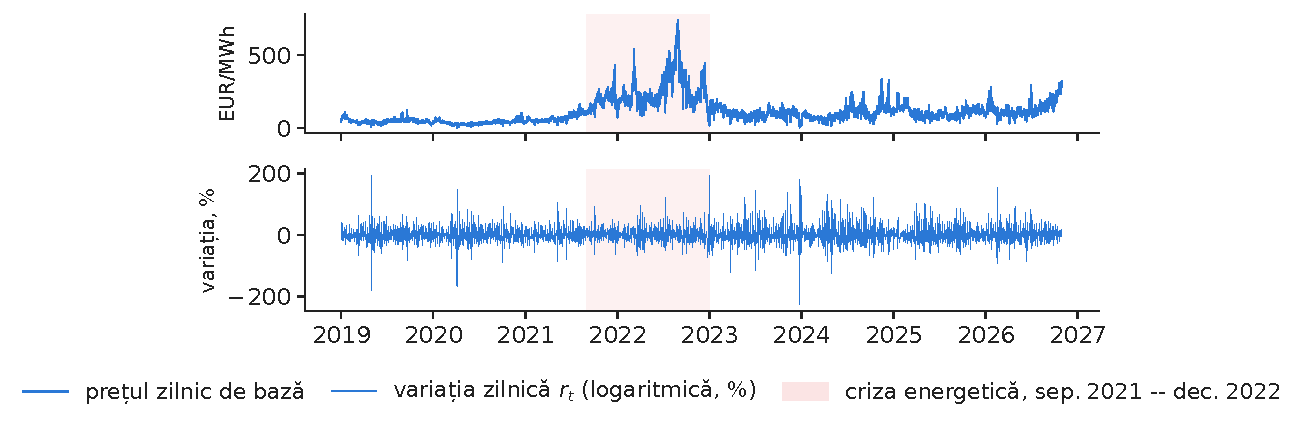
\includegraphics[width=\textwidth,height=0.480\textheight,keepaspectratio]{charts/ro/returns_ro.pdf}\end{center}\vspace{-3mm}
\chartsource{Sursa: energy-charts.info (Fraunhofer ISE); prețurile PZU (OPCOM), prin ENTSO-E. Date: date zilnice, 2019-01-01 - 2026-10-31, zile de livrare CET.}
\vspace{0.5mm}
\begin{itemize}\setlength{\itemsep}{0pt}
  \item Zilele extreme
    \begin{itemize}\setlength{\itemsep}{0pt}
      \item Creșterea maximă: \ensuremath{+}194\%, la 2 ianuarie 2023; scăderea maximă: \ensuremath{-}227\%, la 25 decembrie 2023 (Crăciunul)
      \item 189 de zile cu $|r_t|>50\%$, din 2\,860
    \end{itemize}
\end{itemize}
\par\vfill\manager{o lună calmă spune puțin despre luna următoare: riscul apare grupat.}\par\vspace{0.5mm}
\par\vfill\noindent{\scriptsize\color{FooterGray}(prețurile PZU publicate de OPCOM)}\hfill\qlink{EMQA\_L3\_returns\_ro}{Quantlets/L3/EMQA_L3_returns_ro}\par\vspace{0.5mm}
\end{frame}

\begin{frame}{Lîngă zero, variația procentuală explodează; sub zero, nu există}
\footnotesize
\intuition{Logaritmul cere prețuri pozitive; lîngă zero, variații obișnuite devin procente uriașe.}
\begin{columns}[T,onlytextwidth]
\begin{column}{0.52\textwidth}
\[ \operatorname{asinh}(x)=\ln\bigl(x+\sqrt{x^2+1}\bigr) \]\vspace{-2mm}\[ \Delta\operatorname{asinh}P_t\approx\Delta\ln P_t\ \ \text{dacă}\ P_t\gg 1 \]{\footnotesize\begin{itemize}\setlength{\itemsep}{0pt}
  \item \textbf{\txtwhere}
    \begin{itemize}\setlength{\itemsep}{0pt}
      \item $\operatorname{asinh}$ = sinusul hiperbolic invers, definit pentru orice semn
      \item De la 100 la 120 EUR/MWh ambele formule dau 18{,}2\%
      \item Lîngă zero ambele explodează.
    \end{itemize}
\end{itemize}\par}
\end{column}
\begin{column}{0.45\textwidth}
\begin{itemize}\setlength{\itemsep}{1pt}
  \item \textbf{Pe datele noastre}, 2019--2026
    \begin{itemize}\setlength{\itemsep}{0pt}
      \item România: prețul de bază a fost mereu pozitiv (minimum 3{,}97 EUR/MWh)
      \item Dar 485 de ore cu prețuri negative, în 117 zile
      \item DE-LU: 20 de zile cu prețul de bază $\le 0$; de la 0{,}95 la 92{,}91 EUR/MWh: $r_t$ = 458\%
    \end{itemize}
  \item \textbf{Alegerea din acest curs}
    \begin{itemize}\setlength{\itemsep}{0pt}
      \item Prețul de bază: $r_t$ (\%) și $\Delta P_t$ (EUR/MWh); prețurile orare: EUR/MWh
    \end{itemize}
\end{itemize}
\end{column}
\end{columns}
\par\vfill\manager{o poziție se măsoară în MWh, deci riscul ei este în EUR/MWh
    \begin{itemize}\setlength{\itemsep}{0pt}
      \item Procentele au sens doar departe de zero.
    \end{itemize}}\par\vspace{0.5mm}
\par\vfill\noindent{\scriptsize\color{FooterGray}(Uniejewski, Weron \& Ziel, 2018, IEEE TPWRS)}\hfill\tryit{notebook-ul Jupyter, secțiunea 1}\par\vspace{0.5mm}
\end{frame}

\begin{frame}{Jumătate din variația zilnică vine din calendarul săptămînal}
\small
\vspace{-1mm}\[ r_t=c+\textstyle\sum_{k=1}^{7}\phi_k r_{t-k}+\sum_{j=2}^{7}\delta_j D_{j,t}+\varepsilon_t \]\vspace{-2mm}
\begin{center}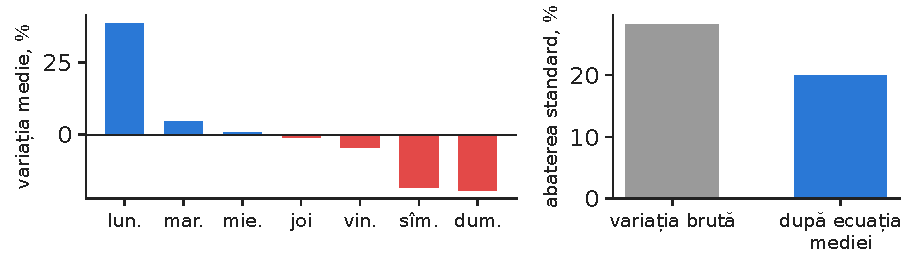
\includegraphics[width=\textwidth,height=0.423\textheight,keepaspectratio]{charts/ro/dow_effect.pdf}\end{center}\vspace{-3mm}
\chartsource{Sursa: energy-charts.info (Fraunhofer ISE); prețurile PZU (OPCOM), prin ENTSO-E. Date: date zilnice, 2019-01-01 - 2026-10-31.}
\vspace{0.5mm}
\begin{itemize}\setlength{\itemsep}{0pt}
  \item Ecuația mediei: $\phi_k$ = ponderea variației de acum $k$ zile; $D_{j,t}=1$ în ziua $j$ a săptămînii; $R^2$ = 0{,}50
    \begin{itemize}\setlength{\itemsep}{0pt}
      \item Abaterea standard scade de la 28{,}3\% la 20{,}0\%; modelele folosesc $\varepsilon_t$ și, în EUR/MWh, $u_t$
    \end{itemize}
\end{itemize}
\par\vfill\manager{creșterea prețului de luni nu este un semnal de risc: ea trebuie prognozată, nu acoperită.}\par\vspace{0.5mm}
\par\vfill\noindent{\scriptsize\color{FooterGray}(estimare proprie; Weron, 2014, IJF)}\hfill\qlink{EMQA\_L3\_dow\_effect}{Quantlets/L3/EMQA_L3_dow_effect}\par\vspace{0.5mm}
\end{frame}

\subsection{Faptele stilizate}

\begin{frame}{Sensul unui șoc nu poate fi anticipat, mărimea lui da}
\small
\begin{center}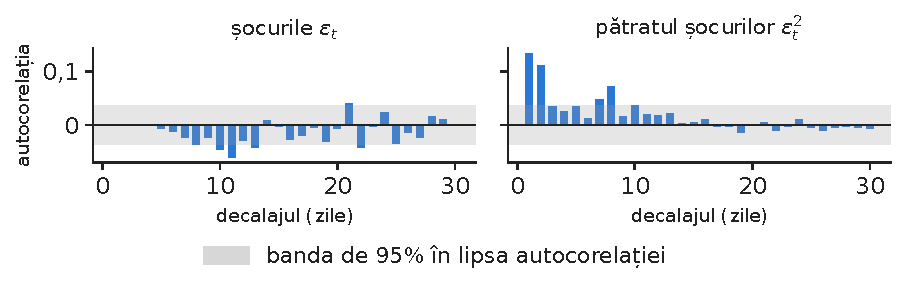
\includegraphics[width=\textwidth,height=0.410\textheight,keepaspectratio]{charts/ro/acf_clust.pdf}\end{center}\vspace{-3mm}
\chartsource{Sursa: energy-charts.info (Fraunhofer ISE); prețurile PZU (OPCOM), prin ENTSO-E. Date: reziduurile ecuației mediei, 2019-01-01 - 2026-10-31.}
\vspace{0.5mm}
\begin{itemize}\setlength{\itemsep}{0pt}
  \item Testul Ljung--Box $Q(10)=T(T+2)\sum_{k\le10}\hat\rho_k^2/(T-k)$, $\hat\rho_k$ = autocorelația de ordin $k$: 13{,}8 pentru $\varepsilon_t$ ($p$ = 0{,}18), 120{,}0 pentru $\varepsilon_t^2$ (valoarea critică: 18{,}31)
    \begin{itemize}\setlength{\itemsep}{0pt}
      \item Testul multiplicatorului Lagrange pentru heteroscedasticitate condiționată autoregresivă (ARCH-LM), 10 decalaje: 93{,}7, $p<0{,}001$
    \end{itemize}
\end{itemize}
\par\vfill\manager{un șoc mare astăzi anunță șocuri mari și în zilele următoare: acesta este subiectul cursului.}\par\vspace{0.5mm}
\par\vfill\noindent{\scriptsize\color{FooterGray}(Ljung \& Box, 1978; Engle, 1982, Econometrica)}\hfill\qlink{EMQA\_L3\_acf\_clust}{Quantlets/L3/EMQA_L3_acf_clust}\par\vspace{0.5mm}
\end{frame}

\begin{frame}{Zilele extreme sînt mult mai frecvente decît prevede legea normală}
\small
\begin{center}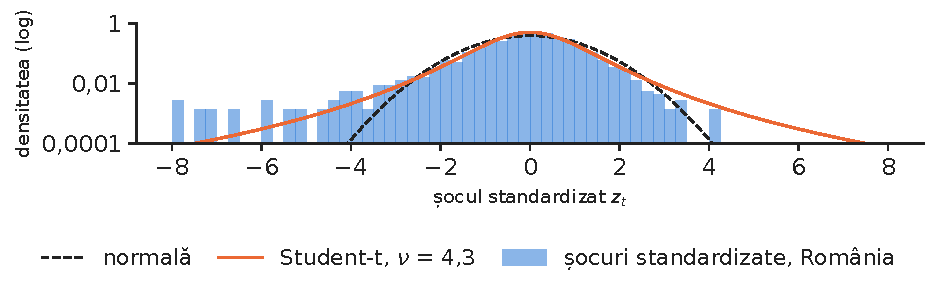
\includegraphics[width=\textwidth,height=0.430\textheight,keepaspectratio]{charts/ro/tails.pdf}\end{center}\vspace{-3mm}
\chartsource{Sursa: energy-charts.info (OPCOM, prin ENTSO-E); estimări proprii. Date: GARCH(1,1)-t pe variațiile procentuale, 2019-01-01 - 2026-10-31.}
\vspace{0.5mm}
\begin{itemize}\setlength{\itemsep}{0pt}
  \item Șocurile $\varepsilon_t$: excesul de aplatizare (kurtosis) 20{,}0, asimetria \ensuremath{-}1{,}69 (scăderi mari: sărbători, zile cu vînt puternic)
    \begin{itemize}\setlength{\itemsep}{0pt}
      \item 15 șocuri dincolo de 4 abateri standard, față de 0{,}18 așteptate în ipoteza normalității; distribuția Student, cu $\nu$ = 4{,}3 grade de libertate
    \end{itemize}
\end{itemize}
\par\vfill\manager{o limită calculată cu distribuția normală este depășită mult mai des decît s-a planificat (cursul 4).}\par\vspace{0.5mm}
\par\vfill\noindent{\scriptsize\color{FooterGray}(estimare proprie; Bollerslev, 1987, RESTAT)}\hfill\qlink{EMQA\_L3\_tails}{Quantlets/L3/EMQA_L3_tails}\par\vspace{0.5mm}
\end{frame}

\begin{frame}{Criza: aceeași volatilitate în procente, de 4 ori mai mare în EUR/MWh}
\small
\begin{center}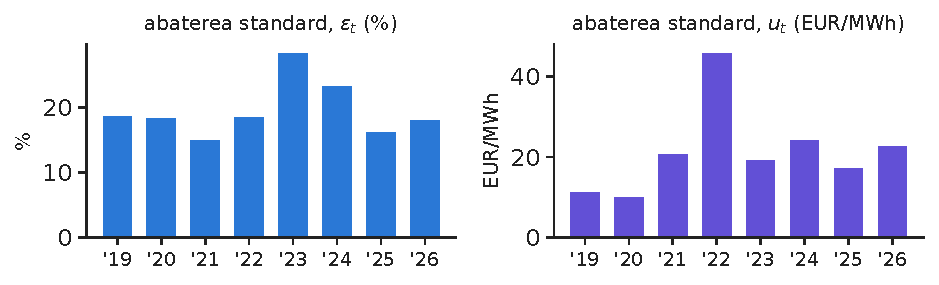
\includegraphics[width=\textwidth,height=0.430\textheight,keepaspectratio]{charts/ro/vol_units.pdf}\end{center}\vspace{-3mm}
\chartsource{Sursa: energy-charts.info (Fraunhofer ISE); prețurile PZU (OPCOM), prin ENTSO-E. Date: reziduurile ecuației mediei, 2019-01-01 - 2026-10-31.}
\vspace{0.5mm}
\begin{itemize}\setlength{\itemsep}{0pt}
  \item Abaterea standard a șocurilor, 2019 față de 2022
    \begin{itemize}\setlength{\itemsep}{0pt}
      \item În procente: 18{,}7\% față de 18{,}5\% (raport 0{,}99)
      \item În EUR/MWh: 11{,}2 față de 45{,}8 (raport 4{,}1); prețul mediu: 50, respectiv 265 EUR/MWh
    \end{itemize}
\end{itemize}
\par\vfill\manager{apelurile în marjă se plătesc în euro: garanțiile au crescut odată cu nivelul prețului, deși volatilitatea procentuală nu a crescut.}\par\vspace{0.5mm}
\par\vfill\noindent{\scriptsize\color{FooterGray}(estimare proprie)}\hfill\qlink{EMQA\_L3\_vol\_units}{Quantlets/L3/EMQA_L3_vol_units}\par\vspace{0.5mm}
\end{frame}

\begin{frame}{Energia electrică este de circa 9 ori mai volatilă decît petrolul}
\footnotesize
\begin{center}{\footnotesize\renewcommand{\arraystretch}{1.05}\setlength{\tabcolsep}{4pt}
\begin{tabular}{@{}lrrrrrrrr@{}}\toprule
Volatilitatea anualizată, \% & 2019 & 2020 & 2021 & 2022 & 2023 & 2024 & 2025 & 2026 \\ \midrule
Energie electrică, România & \cellcolor{Crimson!43}358 & \cellcolor{Crimson!41}349 & \cellcolor{Crimson!23}287 & \cellcolor{Crimson!42}354 & \cellcolor{Crimson!55}543 & \cellcolor{Crimson!55}444 & \cellcolor{Crimson!29}310 & \cellcolor{Crimson!40}346 \\
Energie electrică, Ungaria & \cellcolor{Crimson!12}247 & \cellcolor{Crimson!35}329 & \cellcolor{Crimson!23}289 & \cellcolor{Crimson!37}335 & \cellcolor{Crimson!55}566 & \cellcolor{Crimson!55}547 & \cellcolor{Crimson!43}358 & \cellcolor{Crimson!38}339 \\
EUA & -- & -- & -- & \cellcolor{Forest!44}53 & \cellcolor{Forest!50}32 & \cellcolor{Forest!48}37 & \cellcolor{Forest!52}24 & \cellcolor{Forest!51}28 \\
Brent & \cellcolor{Forest!50}30 & \cellcolor{Forest!39}71 & \cellcolor{Forest!50}32 & \cellcolor{Forest!46}46 & \cellcolor{Forest!50}31 & \cellcolor{Forest!52}25 & \cellcolor{Forest!50}29 & \cellcolor{Forest!43}56 \\
Gaze TTF (lunar) & \cellcolor{Forest!47}42 & \cellcolor{Forest!35}82 & \cellcolor{Forest!42}58 & \cellcolor{Forest!30}100 & \cellcolor{Forest!37}78 & \cellcolor{Forest!48}38 & \cellcolor{Forest!51}28 & \cellcolor{Forest!41}63 \\
OMV Petrom (SNP) & \cellcolor{Forest!52}24 & \cellcolor{Forest!49}35 & \cellcolor{Forest!52}22 & \cellcolor{Forest!52}22 & \cellcolor{Forest!54}18 & \cellcolor{Forest!54}17 & \cellcolor{Forest!53}20 & \cellcolor{Forest!53}21 \\
Hidroelectrica (H2O) & -- & -- & -- & -- & \cellcolor{Forest!55}13 & \cellcolor{Forest!55}14 & \cellcolor{Forest!55}14 & \cellcolor{Forest!50}30 \\
\bottomrule\end{tabular}}\end{center}\vspace{-1mm}\begin{itemize}\setlength{\itemsep}{1pt}
  \item \textbf{Cum se citește tabelul}
    \begin{itemize}\setlength{\itemsep}{0pt}
      \item Abaterea standard a șocurilor zilnice $\times\sqrt{365}$ pentru energie, $\times\sqrt{252}$ pentru activele bursiere; TTF: medii lunare $\times\sqrt{12}$ (subestimează riscul)
      \item Brent are vîrfuri în 2020 și 2026, carbonul în 2022; -- = seria nu era încă disponibilă
    \end{itemize}
\end{itemize}
\par\vfill\manager{nu comparați limitele unui birou de tranzacționare a energiei electrice cu cele ale unui birou de petrol, exprimate în același procent.}\par\vspace{0.5mm}
\par\vfill\noindent{\scriptsize\color{FooterGray}(estimare proprie; Banca Mondială, Pink Sheet)}\hfill\tryit{notebook-ul Jupyter, secțiunea 2}\par\vspace{0.5mm}
\end{frame}


\section{Modelele din familia GARCH}

\subsection{Modelul GARCH(1,1) și estimarea lui}

\begin{frame}{GARCH actualizează varianța de mîine pe baza șocului de azi}
\footnotesize
\intuition{Un șoc mare ieri mărește varianța de azi; efectul se stinge apoi treptat, de la o zi la alta.}
\begin{columns}[T,onlytextwidth]
\begin{column}{0.58\textwidth}
\[ \sigma_t^2=\underbrace{\omega}_{\text{constanta}}+\underbrace{\alpha\,\varepsilon_{t-1}^2}_{\text{reacția la șoc}}+\underbrace{\beta\,\sigma_{t-1}^2}_{\text{memoria}} \]\vspace{-1mm}\[ \varepsilon_t=\sigma_t z_t,\qquad \bar\sigma^2=\frac{\omega}{1-\alpha-\beta} \]{\footnotesize\begin{itemize}\setlength{\itemsep}{0pt}
  \item \textbf{\txtwhere}
    \begin{itemize}\setlength{\itemsep}{0pt}
      \item $\sigma_t^2$ = varianța condiționată, cunoscută în seara zilei $t-1$
      \item $z_t$ = șocul standardizat (media 0, varianța 1)
      \item $\omega>0$, $\alpha,\beta\ge0$, persistența $\alpha+\beta<1$, varianța de lungă durată $\bar\sigma^2$
      \item $\beta=0$: modelul ARCH (Engle, 1982).
    \end{itemize}
\end{itemize}\par}
\end{column}
\begin{column}{0.39\textwidth}
\begin{itemize}\setlength{\itemsep}{1pt}
  \item \textbf{România, șocuri în \%}
    \begin{itemize}\setlength{\itemsep}{0pt}
      \item $\hat\alpha$ = 0{,}308, $\hat\beta$ = 0{,}438, $\hat\alpha+\hat\beta$ = 0{,}746
      \item $\bar\sigma$ de lungă durată: 20{,}4\% pe zi
    \end{itemize}
  \item \textbf{România, șocuri în EUR/MWh}
    \begin{itemize}\setlength{\itemsep}{0pt}
      \item $\hat\alpha$ = 0{,}102, $\hat\beta$ = 0{,}892, $\hat\alpha+\hat\beta$ = 0{,}994
      \item $\bar\sigma$ de lungă durată: 27{,}6 EUR/MWh pe zi
    \end{itemize}
\end{itemize}
\end{column}
\end{columns}
\par\vfill\manager{în fiecare seară, GARCH dă departamentului de risc valoarea $\sigma$ pentru ziua următoare.}\par\vspace{0.5mm}
\par\vfill\noindent{\scriptsize\color{FooterGray}(Engle, 1982, Econometrica; Bollerslev, 1986, JOE)}\hfill\tryit{notebook-ul Jupyter, secțiunea 3}\par\vspace{0.5mm}
\end{frame}

\begin{frame}{Parametrii se estimează prin verosimilitate maximă, cu șocuri Student}
\footnotesize
\intuition{Alegem parametrii care fac cel mai probabile șocurile observate; legea Student lasă loc zilelor extreme.}
\begin{columns}[T,onlytextwidth]
\begin{column}{0.50\textwidth}
\[ \ell(\omega,\alpha,\beta,\nu)=\sum_{t=1}^{T}\Bigl[\ln f_\nu\Bigl(\frac{\varepsilon_t}{\sigma_t}\Bigr)-\ln\sigma_t\Bigr] \]{\footnotesize\begin{itemize}\setlength{\itemsep}{0pt}
  \item \textbf{\txtwhere}
    \begin{itemize}\setlength{\itemsep}{0pt}
      \item $f_\nu$ = densitatea Student cu varianța 1 și $\nu>2$ grade de libertate
      \item $\nu$ mic = cozi groase, $\nu\to\infty$ = distribuția normală
      \item Criteriul informațional bayesian (BIC) $=k\ln T-2\hat\ell$, $k$ = numărul de parametri (mai mic = mai bun)
      \item Anexa A.
    \end{itemize}
\end{itemize}\par}
\end{column}
\begin{column}{0.47\textwidth}
{\footnotesize\renewcommand{\arraystretch}{1.15}\setlength{\tabcolsep}{4pt}
\begin{tabular}{@{}lrr@{}}\toprule
GARCH(1,1), șocuri în \% & normală & Student \\ \midrule
log-verosimilitatea & \ensuremath{-}12\,360{,}3 & \ensuremath{-}12\,094{,}5 \\
BIC & 24\,744{,}5 & 24\,220{,}8 \\
$\hat\alpha+\hat\beta$ & 0{,}927 & 0{,}746 \\
înjumătățire, zile & 9{,}2 & 2{,}4 \\
$\hat\nu$ & -- & 4{,}27 \\
\bottomrule\end{tabular}}\begin{itemize}\setlength{\itemsep}{1pt}
  \item \textbf{Interpretare}
    \begin{itemize}\setlength{\itemsep}{0pt}
      \item Modelul Student cîștigă (BIC mai mic); cel normal tratează fiecare sărbătoare ca volatilitate durabilă
    \end{itemize}
\end{itemize}
\end{column}
\end{columns}
\par\vfill\manager{folosiți șocuri de tip Student
    \begin{itemize}\setlength{\itemsep}{0pt}
      \item Cu șocuri normale, limitele rămîn largi prea mult timp.
    \end{itemize}}\par\vspace{0.5mm}
\par\vfill\noindent{\scriptsize\color{FooterGray}(Bollerslev, 1987, RESTAT)}\hfill\tryit{notebook-ul Jupyter, secțiunea 3}\par\vspace{0.5mm}
\end{frame}

\begin{frame}{GARCH: salturi scurte în procente, valori mari durabile în EUR/MWh}
\small
\begin{center}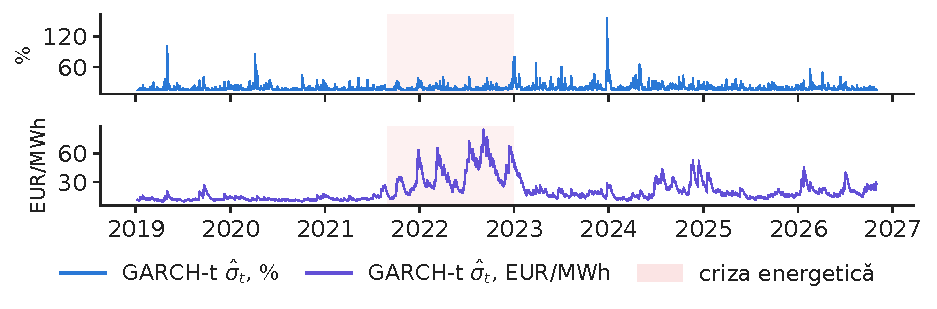
\includegraphics[width=\textwidth,height=0.515\textheight,keepaspectratio]{charts/ro/cond_vol.pdf}\end{center}\vspace{-3mm}
\chartsource{Sursa: energy-charts.info (OPCOM, prin ENTSO-E); estimări proprii. Date: GARCH(1,1)-t, 2019-01-01 - 2026-10-31.}
\vspace{0.5mm}
\begin{itemize}\setlength{\itemsep}{0pt}
  \item Valorile maxime
    \begin{itemize}\setlength{\itemsep}{0pt}
      \item În procente: 156\% pe zi, la 26 decembrie 2023, dispărute în cîteva zile
      \item În EUR/MWh: 85{,}7, la 4 septembrie 2022, față de un minim de 8{,}8, la 6 iulie 2019; 27{,}4 la sfîrșitul perioadei
    \end{itemize}
\end{itemize}
\par\vfill\manager{garanțiile unui furnizor urmează curba în EUR/MWh, nu pe cea procentuală.}\par\vspace{0.5mm}
\par\vfill\noindent{\scriptsize\color{FooterGray}(estimare proprie, GARCH(1,1)-t)}\hfill\qlink{EMQA\_L3\_cond\_vol}{Quantlets/L3/EMQA_L3_cond_vol}\par\vspace{0.5mm}
\end{frame}

\subsection{Persistența și timpul de înjumătățire}

\begin{frame}{Timpul de înjumătățire arată în cîte zile dispare jumătate din șoc}
\footnotesize
\intuition{Varianța suplimentară creată de un șoc se reduce în fiecare zi cu factorul $\alpha+\beta$.}
\begin{columns}[T,onlytextwidth]
\begin{column}{0.49\textwidth}
\[ \E_t\bigl[\sigma^2_{t+h}\bigr]-\bar\sigma^2=(\alpha+\beta)^{h-1}\bigl(\sigma^2_{t+1}-\bar\sigma^2\bigr) \]\vspace{-1mm}\[ h_{1/2}=\frac{\ln 0{,}5}{\ln(\alpha+\beta)} \]{\footnotesize\begin{itemize}\setlength{\itemsep}{0pt}
  \item \textbf{\txtwhere}
    \begin{itemize}\setlength{\itemsep}{0pt}
      \item $\E_t$ = media condiționată de datele pînă în ziua $t$
      \item $h$ = numărul de zile
      \item $h_{1/2}$ = timpul de înjumătățire
      \item Deducerea formulei: anexa B.
    \end{itemize}
\end{itemize}\par}
\end{column}
\begin{column}{0.48\textwidth}
{\footnotesize\renewcommand{\arraystretch}{1.12}\setlength{\tabcolsep}{4pt}
\begin{tabular}{@{}lrrl@{}}\toprule
GARCH(1,1)-t & $\hat\alpha+\hat\beta$ & $h_{1/2}$ & unitatea \\ \midrule
România, \% & 0{,}746 & 2{,}4 & zile \\
România, EUR/MWh & 0{,}994 & 113{,}5 & zile \\
Ungaria, \% & 0{,}881 & 5{,}5 & zile \\
Brent & 0{,}973 & 25{,}6 & zile lucrătoare \\
EUA & 0{,}992 & 82{,}8 & zile lucrătoare \\
OMV Petrom & 0{,}934 & 10{,}2 & zile lucrătoare \\
\bottomrule\end{tabular}}
\par\vspace{0.5mm}{\scriptsize \begin{itemize}\setlength{\itemsep}{0pt}
  \item Eșantioane: energie electrică și Brent din 2019, EUA din 19 octombrie 2021, OMV Petrom din 2019.
\end{itemize}}
\end{column}
\end{columns}
\par\vfill\manager{după un șoc pe piața petrolului, mențineți limite mai largi circa 5 săptămîni
    \begin{itemize}\setlength{\itemsep}{0pt}
      \item După un șoc procentual al prețului energiei electrice, doar cîteva zile.
    \end{itemize}}\par\vspace{0.5mm}
\par\vfill\noindent{\scriptsize\color{FooterGray}(Engle, 2001, JEP)}\hfill\tryit{notebook-ul Jupyter, secțiunea 3}\par\vspace{0.5mm}
\end{frame}

\begin{frame}{Petrolul și carbonul: șocurile de volatilitate durează săptămîni}
\small
\begin{center}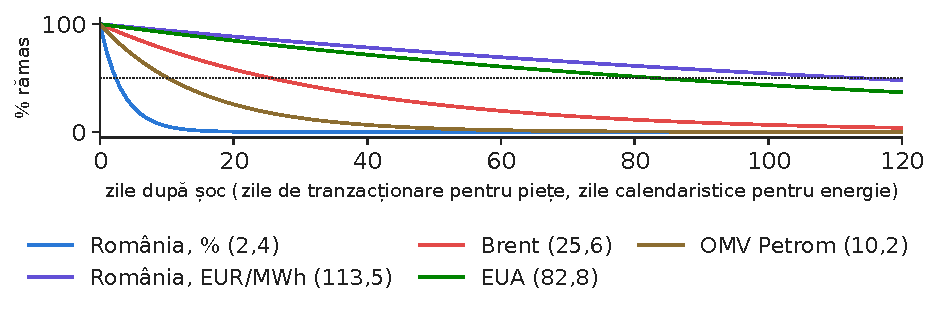
\includegraphics[width=\textwidth,height=0.467\textheight,keepaspectratio]{charts/ro/halflife.pdf}\end{center}\vspace{-3mm}
\chartsource{Sursa: energy-charts.info (OPCOM, prin ENTSO-E); Yahoo Finance (Brent BZ=F, titlul SparkChange EUA ETC); EODHD (acțiuni BVB). Date: GARCH(1,1)-t, fiecare serie pe propriul eșantion (tabelul de pe diapozitiv).}
\vspace{0.5mm}
\begin{itemize}\setlength{\itemsep}{0pt}
  \item Curbele: $100(\hat\alpha+\hat\beta)^h$ = varianța suplimentară rămasă (\%) după $h$ zile; în paranteze: $h_{1/2}$
    \begin{itemize}\setlength{\itemsep}{0pt}
      \item Brent: 26 de zile lucrătoare, circa 5 săptămîni; EUA: 83, circa 17 săptămîni
      \item România: 2{,}4 zile în procente, dar 114 de zile în EUR/MWh, unde volatilitatea urmează nivelul prețului
    \end{itemize}
\end{itemize}
\par\vfill\manager{după un șoc, limitele rămîn mai largi săptămîni, nu zile, cum anunța cursul 1.}\par\vspace{0.5mm}
\par\vfill\noindent{\scriptsize\color{FooterGray}(estimare proprie)}\hfill\qlink{EMQA\_L3\_halflife}{Quantlets/L3/EMQA_L3_halflife}\par\vspace{0.5mm}
\end{frame}

\subsection{Asimetria}

\begin{frame}{GARCH asimetric: creșterile și scăderile nu au același efect}
\footnotesize
\intuition{Două extensii permit ca o creștere și o scădere de aceeași mărime să aibă efecte diferite asupra varianței de mîine.}
\begin{columns}[T,onlytextwidth]
\begin{column}{0.52\textwidth}
\[ \text{GJR:}\ \ \sigma_t^2=\omega+(\alpha+\gamma I_{t-1})\varepsilon_{t-1}^2+\beta\sigma_{t-1}^2 \]\[ \text{EGARCH:}\ \ \ln\sigma_t^2=\omega+\alpha\bigl(|z_{t-1}|-\sqrt{2/\pi}\bigr)+\gamma z_{t-1}+\beta\ln\sigma_{t-1}^2 \]{\footnotesize\begin{itemize}\setlength{\itemsep}{0pt}
  \item \textbf{\txtwhere}
    \begin{itemize}\setlength{\itemsep}{0pt}
      \item $I_{t-1}=1$ dacă $\varepsilon_{t-1}<0$, altfel 0
      \item Modelul Glosten--Jagannathan--Runkle (GJR): $\gamma>0$ = scăderile cresc mai mult volatilitatea (efectul de levier al acțiunilor), $\gamma<0$ = creșterile
      \item GARCH exponențial (EGARCH): convenția de semn pentru $\gamma$ este inversă.
    \end{itemize}
\end{itemize}\par}
\end{column}
\begin{column}{0.45\textwidth}
\begin{itemize}\setlength{\itemsep}{1pt}
  \item \textbf{România, șocuri în \%}
    \begin{itemize}\setlength{\itemsep}{0pt}
      \item GJR: $\hat\gamma$ = 0{,}225 ($t$ = 2{,}9); EGARCH: $\hat\gamma$ = \ensuremath{-}0{,}083 ($t$ = \ensuremath{-}3{,}9)
      \item Scăderile cresc mai mult volatilitatea (revenire după scădere)
    \end{itemize}
  \item \textbf{România, șocuri în EUR/MWh}
    \begin{itemize}\setlength{\itemsep}{0pt}
      \item GJR: $\hat\gamma$ = \ensuremath{-}0{,}127 ($t$ = \ensuremath{-}6{,}4); EGARCH: $\hat\gamma$ = 0{,}104 ($t$ = 7{,}2)
      \item Creșterile cresc mai mult volatilitatea: efectul de levier invers
    \end{itemize}
\end{itemize}
\end{column}
\end{columns}
\par\vfill\manager{pentru un cumpărător, direcția periculoasă este în sus: după un salt de preț, lărgiți limitele mai mult decît după o scădere.}\par\vspace{0.5mm}
\par\vfill\noindent{\scriptsize\color{FooterGray}(Glosten et al., 1993, JFIN; Nelson, 1991; Knittel \& Roberts, 2005, ENEECO)}\hfill\tryit{notebook-ul Jupyter, secțiunea 4}\par\vspace{0.5mm}
\end{frame}

\begin{frame}{În EUR/MWh, creșterile de preț măresc mai mult volatilitatea}
\small
\begin{center}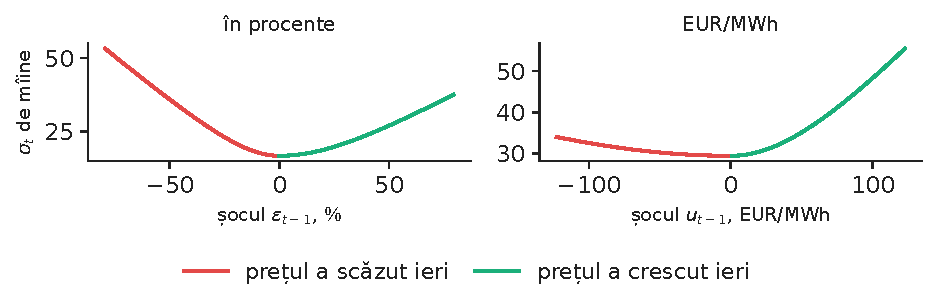
\includegraphics[width=\textwidth,height=0.434\textheight,keepaspectratio]{charts/ro/nic.pdf}\end{center}\vspace{-3mm}
\chartsource{Sursa: energy-charts.info (OPCOM, prin ENTSO-E); estimări proprii. Date: GJR(1,1)-t, 2019-01-01 - 2026-10-31.}
\vspace{0.5mm}
\begin{itemize}\setlength{\itemsep}{0pt}
  \item Curba de impact a șocurilor: $\sigma$ de mîine în funcție de șocul de azi (GJR); pentru un șoc de 61 EUR/MWh
    \begin{itemize}\setlength{\itemsep}{0pt}
      \item $\sigma$ în ziua următoare: 37{,}6 EUR/MWh după o creștere, 30{,}6 după o scădere
      \item În procente (șoc de 40\%), ordinea se inversează: 30{,}3\% după o scădere, 23{,}7\% după o creștere
    \end{itemize}
\end{itemize}
\par\vfill\manager{un consumator industrial care cumpără la prețul spot trebuie să reacționeze mai repede la creșteri decît la scăderi.}\par\vspace{0.5mm}
\par\vfill\noindent{\scriptsize\color{FooterGray}(Engle \& Ng, 1993, JFIN; estimare proprie, GJR(1,1)-t)}\hfill\qlink{EMQA\_L3\_nic}{Quantlets/L3/EMQA_L3_nic}\par\vspace{0.5mm}
\end{frame}

\begin{frame}{Volatilitatea în EUR/MWh crește odată cu nivelul prețului}
\small
\begin{center}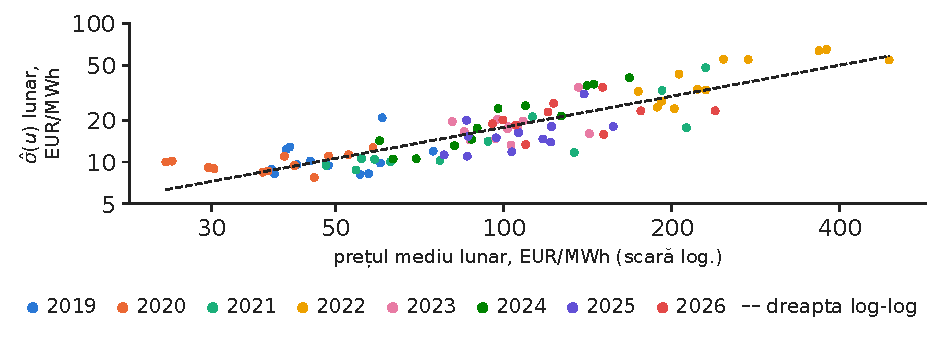
\includegraphics[width=\textwidth,height=0.480\textheight,keepaspectratio]{charts/ro/vol_level.pdf}\end{center}\vspace{-3mm}
\chartsource{Sursa: energy-charts.info (Fraunhofer ISE); prețurile PZU (OPCOM), prin ENTSO-E. Date: date lunare, 2019-01-01 - 2026-10-31.}
\vspace{0.5mm}
\begin{itemize}\setlength{\itemsep}{0pt}
  \item Explicația: la prețuri mari, curba ofertei (ordinea de merit) este mai abruptă, deci același șoc al cererii mută mai mult prețul
    \begin{itemize}\setlength{\itemsep}{0pt}
      \item Regresia lui $\ln\hat\sigma_m(u)$ pe $\ln\bar P_m$, 94 de luni: panta 0{,}75, $R^2$ = 0{,}76; în procente: panta 0{,}01, $R^2$ = 0{,}00
    \end{itemize}
\end{itemize}
\par\vfill\manager{stabiliți limitele în EUR/MWh ca procent din prețul contractelor la termen, nu ca sumă fixă.}\par\vspace{0.5mm}
\par\vfill\noindent{\scriptsize\color{FooterGray}(Knittel \& Roberts, 2005, ENEECO; estimare proprie)}\hfill\qlink{EMQA\_L3\_vol\_level}{Quantlets/L3/EMQA_L3_vol_level}\par\vspace{0.5mm}
\end{frame}

\begin{frame}{Cozile groase contează mai mult decît asimetria}
\footnotesize
\begin{center}{\footnotesize\renewcommand{\arraystretch}{1.05}\setlength{\tabcolsep}{4pt}
\begin{tabular}{@{}lrrrrrr@{}}\toprule
Modelul & $\alpha+\beta$ (\%) & BIC (\%) & $p$, $z^2$ (\%) & $\alpha+\beta$ (EUR) & BIC (EUR) & $p$, $z^2$ (EUR) \\ \midrule
GARCH, normal & 0{,}927 & \cellcolor{Crimson!55}24\,744{,}5 & 0{,}328 & 0{,}998 & \cellcolor{Crimson!55}24\,573{,}2 & 0{,}000 \\
GARCH, Student & 0{,}746 & \cellcolor{Forest!54}24\,220{,}8 & 0{,}367 & 0{,}994 & \cellcolor{Forest!25}24\,450{,}7 & 0{,}000 \\
GJR, normal & 0{,}651 & \cellcolor{Crimson!44}24\,690{,}7 & 0{,}151 & 0{,}998 & \cellcolor{Crimson!24}24\,525{,}1 & 0{,}000 \\
GJR, Student & 0{,}727 & \cellcolor{Forest!55}24\,214{,}1 & 0{,}243 & 0{,}996 & \cellcolor{Forest!50}24\,411{,}7 & 0{,}000 \\
EGARCH, normal & 0{,}903 & \cellcolor{Crimson!44}24\,691{,}4 & 0{,}529 & 0{,}995 & \cellcolor{Crimson!19}24\,518{,}0 & 0{,}000 \\
EGARCH, Student & 0{,}831 & \cellcolor{Forest!54}24\,219{,}2 & 0{,}532 & 0{,}995 & \cellcolor{Forest!55}24\,403{,}9 & 0{,}000 \\
\bottomrule\end{tabular}}\end{center}\vspace{-1mm}\begin{itemize}\setlength{\itemsep}{1pt}
  \item \textbf{Clasamentul după BIC} (verde = cel mai bun)
    \begin{itemize}\setlength{\itemsep}{0pt}
      \item Orice model cu distribuția Student îl depășește pe oricare cu distribuția normală; cel mai bun: GJR-t în \%, EGARCH-t în EUR/MWh; criteriul informațional Akaike (AIC): anexa C
    \end{itemize}
  \item \textbf{Diagnostic}: valoarea $p$ Ljung--Box pentru $z_t^2$, pătratul șocurilor standardizate
    \begin{itemize}\setlength{\itemsep}{0pt}
      \item În \% nu mai rămîne grupare; în EUR/MWh rămîne ($p<0{,}001$): o singură ecuație nu poate urmări și nivelul prețului, și șocurile zilnice
    \end{itemize}
\end{itemize}
\par\vfill\manager{mai întîi modelați corect cozile distribuției, apoi asimetria.}\par\vspace{0.5mm}
\par\vfill\noindent{\scriptsize\color{FooterGray}(Bollerslev, 1987; Glosten, Jagannathan \& Runkle, 1993; Nelson, 1991)}\hfill\tryit{notebook-ul Jupyter, secțiunea 4}\par\vspace{0.5mm}
\end{frame}


\section{Regimuri de volatilitate și criza energetică}

\begin{frame}{Modelul Markov cu schimbare de regim separă calmul de agitație}
\footnotesize
\intuition{Două stări neobservate, fiecare cu volatilitatea ei; pentru fiecare zi, modelul dă probabilitatea stării agitate.}
\begin{columns}[T,onlytextwidth]
\begin{column}{0.52\textwidth}
\[ u_t=\mu_{s_t}+\sigma_{s_t}\eta_t,\qquad \Pr(s_t=j\mid s_{t-1}=i)=p_{ij} \]\vspace{-1mm}\[ \text{durata medie a regimului } i=\frac{1}{1-p_{ii}} \]{\footnotesize\begin{itemize}\setlength{\itemsep}{0pt}
  \item \textbf{\txtwhere}
    \begin{itemize}\setlength{\itemsep}{0pt}
      \item $u_t$ = șocul în EUR/MWh
      \item $s_t$ = regimul (calm sau agitat)
      \item $\eta_t$ = variabilă normală standard
      \item $p_{ij}$ = probabilitățile de tranziție, estimate prin verosimilitate maximă (anexa D).
    \end{itemize}
\end{itemize}\par}
\end{column}
\begin{column}{0.45\textwidth}
\begin{itemize}\setlength{\itemsep}{1pt}
  \item \textbf{România, șocuri în EUR/MWh}
    \begin{itemize}\setlength{\itemsep}{0pt}
      \item Calm: $\sigma$ = 12{,}9, $p_{11}$ = 0{,}986, circa 69 de zile
      \item Agitat: $\sigma$ = 41{,}9, $p_{22}$ = 0{,}957, circa 23 de zile; 24\% din zile
    \end{itemize}
  \item \textbf{În procente}
    \begin{itemize}\setlength{\itemsep}{0pt}
      \item Starea agitată: doar 3{,}5 zile, salturi izolate
    \end{itemize}
\end{itemize}
\end{column}
\end{columns}
\par\vfill\manager{o probabilitate a regimului agitat peste 0{,}5 cere revizuirea acoperirii riscului și a garanțiilor.}\par\vspace{0.5mm}
\par\vfill\noindent{\scriptsize\color{FooterGray}(Hamilton, 1989, Econometrica)}\hfill\tryit{notebook-ul Jupyter, secțiunea 5}\par\vspace{0.5mm}
\end{frame}

\begin{frame}{Criza a fost un regim agitat lung; 2026 alternează între regimuri}
\small
\begin{center}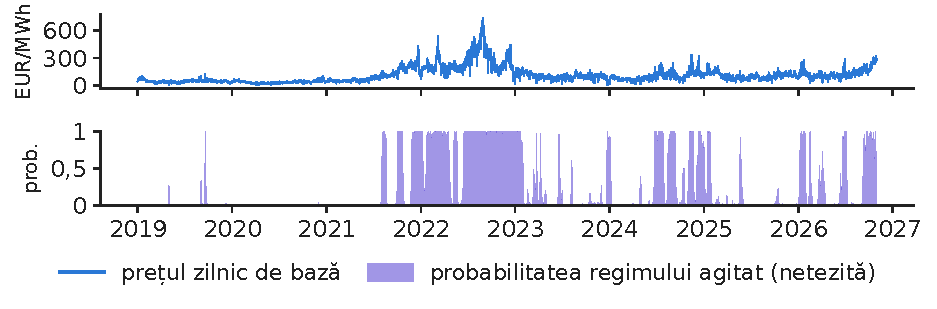
\includegraphics[width=\textwidth,height=0.445\textheight,keepaspectratio]{charts/ro/ms_regime.pdf}\end{center}\vspace{-3mm}
\chartsource{Sursa: energy-charts.info (OPCOM, prin ENTSO-E); estimări proprii. Date: model Markov cu două regimuri, pe șocurile în EUR/MWh, 2019-01-01 - 2026-10-31.}
\vspace{0.5mm}
\begin{itemize}\setlength{\itemsep}{0pt}
  \item Zilele din regimul agitat
    \begin{itemize}\setlength{\itemsep}{0pt}
      \item Cel mai lung episod: 15 iunie 2022 -- 31 ianuarie 2023, 231 de zile
      \item Ponderea pe ani: 2022 86\%, 2025 6\%, 2026 33\% (48\% din iulie)
    \end{itemize}
\end{itemize}
\par\vfill\manager{Transelectrica și furnizorii pot folosi această probabilitate ca avertizare timpurie pentru costurile de echilibrare.}\par\vspace{0.5mm}
\par\vfill\noindent{\scriptsize\color{FooterGray}(estimare proprie; Hamilton, 1989)}\hfill\qlink{EMQA\_L3\_ms\_regime}{Quantlets/L3/EMQA_L3_ms_regime}\par\vspace{0.5mm}
\end{frame}

\begin{frame}{Persistența depinde de perioadă și de unitatea de măsură}
\footnotesize
\begin{center}{\footnotesize\renewcommand{\arraystretch}{1.1}\setlength{\tabcolsep}{4pt}
\begin{tabular}{@{}lrrrrr@{}}\toprule
GARCH(1,1)-t pe & $\hat\alpha+\hat\beta$ (\%) & $h_{1/2}$ (\%) & $\hat\alpha+\hat\beta$ (EUR) & $h_{1/2}$ (EUR) & $\bar\sigma$, EUR/MWh \\ \midrule
2019--2020 (calm) & 0{,}568 & 1{,}2 & 0{,}208 & 0{,}4 & 10{,}5 \\
2021--2022 (criză) & 0{,}882 & 5{,}5 & 1{,}000 & $\infty$ & -- \\
2023 -- octombrie 2026 & 0{,}727 & 2{,}2 & 0{,}927 & 9{,}1 & 20{,}9 \\
întreaga perioadă & 0{,}746 & 2{,}4 & 0{,}994 & 113{,}5 & 27{,}6 \\
\bottomrule\end{tabular}}\end{center}\vspace{-1mm}\begin{itemize}\setlength{\itemsep}{1pt}
  \item \textbf{În EUR/MWh}
    \begin{itemize}\setlength{\itemsep}{0pt}
      \item În 2019--2020 un șoc se înjumătățește în mai puțin de o zi; în criză, $\hat\alpha+\hat\beta$ ajunge la 1, deoarece volatilitatea a crescut lună de lună odată cu prețul
      \item Valoarea pentru întreaga perioadă amestecă regimurile, ceea ce supraestimează persistența
    \end{itemize}
  \item \textbf{În procente}
    \begin{itemize}\setlength{\itemsep}{0pt}
      \item Persistența rămîne mult sub 1 în fiecare perioadă: criza a mutat nivelul prețului, nu volatilitatea procentuală
    \end{itemize}
\end{itemize}
\par\vfill\manager{reestimați modelul după o schimbare de regim
    \begin{itemize}\setlength{\itemsep}{0pt}
      \item Un model estimat pe perioada crizei menține limitele largi prea mult timp.
    \end{itemize}}\par\vspace{0.5mm}
\par\vfill\noindent{\scriptsize\color{FooterGray}(Lamoureux \& Lastrapes, 1990, JBES; estimare proprie)}\hfill\tryit{notebook-ul Jupyter, secțiunea 5}\par\vspace{0.5mm}
\end{frame}


\section{Volatilitatea intrazilnică, din prețurile orare}

\begin{frame}{Variația intrazilnică măsoară cît se mișcă prețul în cursul zilei}
\footnotesize
\intuition{Adunăm pătratele variațiilor de la o oră la alta din aceeași zi de livrare; din această variație cîștigă o baterie sau un consumator flexibil.}
\begin{columns}[T,onlytextwidth]
\begin{column}{0.52\textwidth}
\[ \text{RV}_d=\sqrt{\textstyle\sum_{h=1}^{H_d-1}\bigl(P_{d,h}-P_{d,h-1}\bigr)^2},\qquad \text{relativă}=\frac{\text{RV}_d}{\bar P_d} \]{\footnotesize\begin{itemize}\setlength{\itemsep}{0pt}
  \item \textbf{\txtwhere}
    \begin{itemize}\setlength{\itemsep}{0pt}
      \item $P_{d,h}$ = prețul orei $h$ din ziua $d$ (din 1 octombrie 2025, media celor patru sferturi de oră)
      \item $H_d$ = 24 de ore (23 sau 25 în cele 8 + 8 zile cu schimbarea orei)
      \item $\bar P_d$ = prețul zilnic de bază
      \item În EUR/MWh, deoarece prețurile orare pot fi negative.
    \end{itemize}
\end{itemize}\par}
\end{column}
\begin{column}{0.45\textwidth}
\begin{itemize}\setlength{\itemsep}{1pt}
  \item \textbf{Variația intrazilnică realizată (RV)}, media anuală
    \begin{itemize}\setlength{\itemsep}{0pt}
      \item 2019: 36; 2022: 186; 2026: 135 EUR/MWh
      \item Raportată la preț (mediana): 0{,}64 în 2019, 1{,}24 în 2024
    \end{itemize}
  \item \textbf{Un risc diferit}
    \begin{itemize}\setlength{\itemsep}{0pt}
      \item Corelația dintre RV$_d$ și $|u_t|$: doar 0{,}46
      \item Nu este volatilitatea realizată din finanțe: cele 24 de ore sînt 24 de produse diferite
    \end{itemize}
\end{itemize}
\end{column}
\end{columns}
\par\vfill\manager{venitul unui investitor în baterii depinde de variația intrazilnică, nu de prețul mediu zilnic.}\par\vspace{0.5mm}
\par\vfill\noindent{\scriptsize\color{FooterGray}(Andersen \& Bollerslev, 1998, IER; Weron, 2014, IJF)}\hfill\tryit{notebook-ul Jupyter, secțiunea 6}\par\vspace{0.5mm}
\end{frame}

\begin{frame}{Producția solară a mărit variația prețului în cursul zilei}
\small
\begin{center}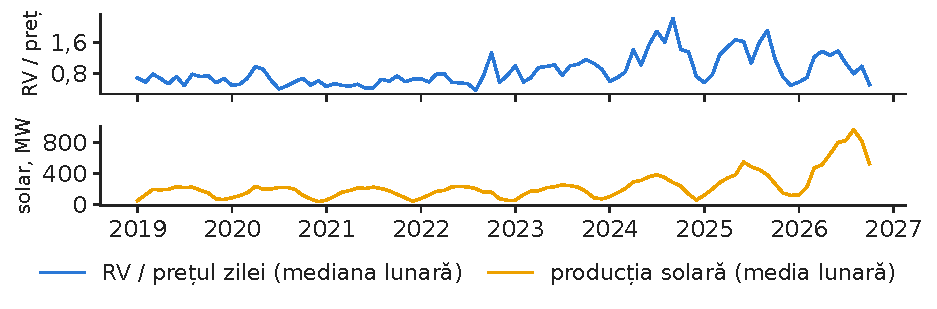
\includegraphics[width=\textwidth,height=0.479\textheight,keepaspectratio]{charts/ro/rv_solar.pdf}\end{center}\vspace{-3mm}
\chartsource{Sursa: energy-charts.info (Fraunhofer ISE); prețuri OPCOM; producția solară ENTSO-E (date Transelectrica pentru România). Date: prețuri orare, valori lunare, 2019-01-01 - 2026-10-31.}
\vspace{0.5mm}
\begin{itemize}\setlength{\itemsep}{0pt}
  \item Variația intrazilnică relativă (mediana)
    \begin{itemize}\setlength{\itemsep}{0pt}
      \item 0{,}64 în 2019, maximum 1{,}24 în 2024, 1{,}01 în 2026
      \item Producția solară medie: 157 MW în 2019, 593 MW în ianuarie -- octombrie 2026; corelația lunară: 0{,}46
    \end{itemize}
\end{itemize}
\par\vfill\manager{mai multă energie solară înseamnă prețuri mici la prînz și mari seara, deci valoare pentru stocare.}\par\vspace{0.5mm}
\par\vfill\noindent{\scriptsize\color{FooterGray}(estimare proprie; producția solară ENTSO-E)}\hfill\qlink{EMQA\_L3\_rv\_solar}{Quantlets/L3/EMQA_L3_rv_solar}\par\vspace{0.5mm}
\end{frame}

\begin{frame}{Variația intrazilnică are memorie lungă: zi, săptămînă, lună}
\footnotesize
\intuition{Trei medii pe orizonturi diferite dau o regresie cu memorie lungă.}
\begin{columns}[T,onlytextwidth]
\begin{column}{0.56\textwidth}
\[ \begin{aligned}\ln\text{RV}_d=b_0&+b_D\ln\text{RV}_{d-1}+\tfrac{b_W}{7}\textstyle\sum_{j=1}^{7}\ln\text{RV}_{d-j}\\ &+\tfrac{b_M}{30}\textstyle\sum_{j=1}^{30}\ln\text{RV}_{d-j}+e_d\end{aligned} \]{\footnotesize\begin{itemize}\setlength{\itemsep}{0pt}
  \item \textbf{\txtwhere}
    \begin{itemize}\setlength{\itemsep}{0pt}
      \item Modelul autoregresiv eterogen (HAR), estimat prin metoda celor mai mici pătrate (OLS)
      \item $b_D$, $b_W$, $b_M$ = ponderile zilei de ieri, ale ultimelor 7 și 30 de zile
      \item Prognoza $=\exp(\widehat{\ln\text{RV}}_d+s^2/2)$, $s^2$ = varianța erorilor.
    \end{itemize}
\end{itemize}\par}
\end{column}
\begin{column}{0.41\textwidth}
\begin{itemize}\setlength{\itemsep}{1pt}
  \item \textbf{Estimări}, înaintea anului de test
    \begin{itemize}\setlength{\itemsep}{0pt}
      \item $\hat b_D$ = 0{,}40, $\hat b_W$ = 0{,}36, $\hat b_M$ = 0{,}22 (toate cu $t>$ 6), $R^2$ = 0{,}82
    \end{itemize}
  \item \textbf{Anul de test}
    \begin{itemize}\setlength{\itemsep}{0pt}
      \item Eroarea absolută medie (MAE): HAR 35{,}6, valoarea de ieri 39{,}1 EUR/MWh (cu 9{,}1\% mai puțin)
    \end{itemize}
\end{itemize}
\end{column}
\end{columns}
\par\vfill\manager{o baterie își programează mentenanța în zilele cu variație prognozată mică.}\par\vspace{0.5mm}
\par\vfill\noindent{\scriptsize\color{FooterGray}(Corsi, 2009, JFEC)}\hfill\tryit{notebook-ul Jupyter, secțiunea 6}\par\vspace{0.5mm}
\end{frame}

\begin{frame}{Prognozele HAR urmăresc variația, dar nu și salturile izolate}
\small
\begin{center}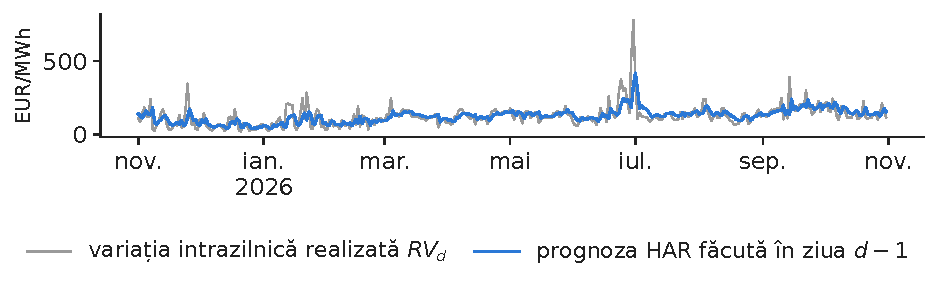
\includegraphics[width=\textwidth,height=0.520\textheight,keepaspectratio]{charts/ro/har_fc.pdf}\end{center}\vspace{-3mm}
\chartsource{Sursa: energy-charts.info (Fraunhofer ISE); prețurile PZU (OPCOM), prin ENTSO-E. Date: anul de test 2025-11-01 - 2026-10-31; HAR reestimat zilnic.}
\vspace{0.5mm}
\begin{itemize}\setlength{\itemsep}{0pt}
  \item Anul de test, prognoză făcută în ziua $d-1$
    \begin{itemize}\setlength{\itemsep}{0pt}
      \item HAR reestimat zilnic pe datele disponibile în ziua $d-1$; MAE 35{,}6 EUR/MWh
    \end{itemize}
\end{itemize}
\par\vfill\manager{folosiți prognoza pentru planificare și păstrați rezerve pentru salturile pe care nu le poate anticipa.}\par\vspace{0.5mm}
\par\vfill\noindent{\scriptsize\color{FooterGray}(estimare proprie)}\hfill\qlink{EMQA\_L3\_har\_fc}{Quantlets/L3/EMQA_L3_har_fc}\par\vspace{0.5mm}
\end{frame}


\section{Prognoza și evaluarea volatilității}

\begin{frame}{Prognoza volatilității se evaluează față de o aproximare zgomotoasă}
\footnotesize
\intuition{Comparăm prognoza cu o aproximare zgomotoasă, pătratul șocului, folosind o funcție de pierdere care ordonează totuși corect modelele.}
\begin{columns}[T,onlytextwidth]
\begin{column}{0.52\textwidth}
\[ \text{QLIKE}_t=\frac{\varepsilon_t^2}{\hat\sigma_t^2}-\ln\frac{\varepsilon_t^2}{\hat\sigma_t^2}-1,\qquad \text{MSE}_t=\bigl(\varepsilon_t^2-\hat\sigma_t^2\bigr)^2 \]{\footnotesize\begin{itemize}\setlength{\itemsep}{0pt}
  \item \textbf{\txtwhere}
    \begin{itemize}\setlength{\itemsep}{0pt}
      \item Funcția de pierdere de tip cvasi-verosimilitate (QLIKE), eroarea pătratică medie (MSE)
      \item $\varepsilon_t$ = șocul zilei $t$, în afara eșantionului
      \item $\hat\sigma_t^2$ = prognoza făcută în $t-1$
      \item MSE este dominată de cîteva zile extreme
      \item Testul Diebold--Mariano (DM) compară pierderile zilnice.
    \end{itemize}
\end{itemize}\par}
\end{column}
\begin{column}{0.45\textwidth}
\begin{itemize}\setlength{\itemsep}{1pt}
  \item \textbf{Exemplu}: $\sigma$ adevărat = 20
    \begin{itemize}\setlength{\itemsep}{0pt}
      \item Prognoza 10: QLIKE = 1{,}61; prognoza 40: QLIKE = 0{,}64
      \item Subestimarea costă de 2{,}5 ori mai mult; MSE spune contrariul
    \end{itemize}
  \item \textbf{Cadrul de evaluare}, anul de test 1 noiembrie 2025 -- 31 octombrie 2026
    \begin{itemize}\setlength{\itemsep}{0pt}
      \item Cinci modele, reestimate zilnic pe datele pînă în $t-1$
    \end{itemize}
\end{itemize}
\end{column}
\end{columns}
\par\vfill\manager{cereți furnizorului modelului de risc valoarea QLIKE pe zilele dumneavoastră, în afara eșantionului.}\par\vspace{0.5mm}
\par\vfill\noindent{\scriptsize\color{FooterGray}(Patton, 2011, JOE; Hansen \& Lunde, 2005, JAE)}\hfill\tryit{notebook-ul Jupyter, secțiunea 7}\par\vspace{0.5mm}
\end{frame}

\begin{frame}{Modelele GARCH sînt mai precise decît varianța istorică}
\footnotesize
\begin{center}{\footnotesize\renewcommand{\arraystretch}{1.05}\setlength{\tabcolsep}{4pt}
\begin{tabular}{@{}lrrrr@{}}\toprule
Varianța pentru ziua următoare & QLIKE, \% & $p$ față de 30 de zile & QLIKE, EUR & $p$ față de 30 de zile \\ \midrule
varianța istorică pe 30 de zile & \cellcolor{Crimson!55}1{,}523 & -- & \cellcolor{Crimson!55}1{,}428 & -- \\
medie cu ponderi exponențiale (EWMA) & \cellcolor{Crimson!21}1{,}499 & 0{,}082 & \cellcolor{Crimson!13}1{,}398 & 0{,}026 \\
GARCH(1,1)-t & \cellcolor{Forest!35}1{,}459 & 0{,}170 & \cellcolor{Forest!15}1{,}378 & 0{,}040 \\
GJR(1,1)-t & \cellcolor{Forest!55}1{,}445 & 0{,}145 & \cellcolor{Forest!44}1{,}357 & 0{,}032 \\
EGARCH(1,1)-t & \cellcolor{Forest!45}1{,}452 & 0{,}120 & \cellcolor{Forest!55}1{,}349 & 0{,}027 \\
\bottomrule\end{tabular}}\end{center}\vspace{-1mm}\begin{itemize}\setlength{\itemsep}{1pt}
  \item \textbf{Interpretare}
    \begin{itemize}\setlength{\itemsep}{0pt}
      \item QLIKE mai mic = model mai bun (verde); $p$ = testul DM unilateral (Newey--West, 7 decalaje), 365 de zile
      \item Cel mai bun: GJR-t în \% (pierdere cu 5{,}1\% sub varianța pe 30 de zile), EGARCH-t în EUR/MWh (5{,}5\%)
    \end{itemize}
  \item \textbf{Semnificația, la pragul de 5\%}
    \begin{itemize}\setlength{\itemsep}{0pt}
      \item În EUR/MWh, toate modelele GARCH sînt mai precise decît varianța istorică; în procente, niciunul; asimetria nu aduce un cîștig semnificativ ($p$ = 0{,}08)
    \end{itemize}
\end{itemize}
\par\vfill\manager{folosiți GARCH-t ca model implicit
    \begin{itemize}\setlength{\itemsep}{0pt}
      \item Modelele asimetrice aduc puțin în afara eșantionului.
    \end{itemize}}\par\vspace{0.5mm}
\par\vfill\noindent{\scriptsize\color{FooterGray}(Diebold \& Mariano, 1995, JBES; Patton, 2011, JOE; RiskMetrics, 1996)}\hfill\tryit{notebook-ul Jupyter, secțiunea 7}\par\vspace{0.5mm}
\end{frame}

\begin{frame}{GARCH reacționează imediat; varianța istorică întîrzie și uită brusc}
\small
\begin{center}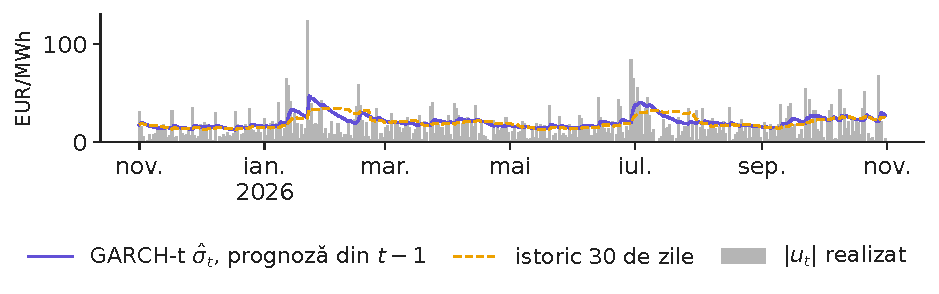
\includegraphics[width=\textwidth,height=0.444\textheight,keepaspectratio]{charts/ro/fc_test.pdf}\end{center}\vspace{-3mm}
\chartsource{Sursa: energy-charts.info (OPCOM, prin ENTSO-E); estimări proprii. Date: anul de test 2025-11-01 - 2026-10-31; modele reestimate zilnic.}
\vspace{0.5mm}
\begin{itemize}\setlength{\itemsep}{0pt}
  \item Cel mai mare șoc din anul de test: \ensuremath{+}124 EUR/MWh, la 22 ianuarie 2026
    \begin{itemize}\setlength{\itemsep}{0pt}
      \item A doua zi, $\hat\sigma$ GARCH crește de la 25 la 47, iar varianța istorică dă doar 33 EUR/MWh
      \item După 30 de zile, șocul iese din fereastră: estimarea istorică scade într-o singură zi de la 32 la 23
    \end{itemize}
\end{itemize}
\par\vfill\manager{o limită care se modifică brusc la 30 de zile după un șoc, fără nicio informație nouă, trădează un model cu fereastră istorică.}\par\vspace{0.5mm}
\par\vfill\noindent{\scriptsize\color{FooterGray}(estimare proprie)}\hfill\qlink{EMQA\_L3\_fc\_test}{Quantlets/L3/EMQA_L3_fc_test}\par\vspace{0.5mm}
\end{frame}

\begin{frame}{Pe mai multe săptămîni, volatilitatea revine spre nivelul normal}
\footnotesize
\intuition{O volatilitate mare se așteaptă să scadă, iar una mică să crească; de aceea, regula $\sigma\sqrt{h}$ greșește riscul pe $h$ zile.}
\begin{columns}[T,onlytextwidth]
\begin{column}{0.52\textwidth}
\[ \hat\sigma^2_{T+h\mid T}=\bar\sigma^2+(\alpha+\beta)^{h-1}\bigl(\hat\sigma^2_{T+1}-\bar\sigma^2\bigr) \]\vspace{-1mm}\[ \Var_T\Bigl(\textstyle\sum_{k=1}^{h}r_{T+k}\Bigr)=\sum_{k=1}^{h}\hat\sigma^2_{T+k\mid T}\ \ne\ h\,\hat\sigma^2_{T+1} \]{\footnotesize\begin{itemize}\setlength{\itemsep}{0pt}
  \item \textbf{\txtwhere}
    \begin{itemize}\setlength{\itemsep}{0pt}
      \item $T$ = ziua prognozei
      \item A doua formulă: randamente fără autocorelație (petrol, carbon), nu energie electrică
      \item Banda de 90\% = $\pm1{,}645\sqrt{\cdot}$.
    \end{itemize}
\end{itemize}\par}
\end{column}
\begin{column}{0.45\textwidth}
\begin{itemize}\setlength{\itemsep}{1pt}
  \item \textbf{Brent la 9 aprilie 2026}, după șocul petrolier din 2026
    \begin{itemize}\setlength{\itemsep}{0pt}
      \item $\hat\sigma_{T+1}$ = 93\% pe an, pe termen lung 39\%
      \item Banda pe 20 de zile: GARCH $\pm$38{,}5\%, $\sigma\sqrt{20}$: $\pm$43{,}1\% (prea largă cu 12\%)
    \end{itemize}
  \item \textbf{Brent la 30 octombrie 2026}, din nou calm
    \begin{itemize}\setlength{\itemsep}{0pt}
      \item $\hat\sigma_{T+1}$ = 32\% $<$ 40\%: acum $\sigma\sqrt{20}$ dă o bandă prea îngustă
    \end{itemize}
\end{itemize}
\end{column}
\end{columns}
\par\vfill\manager{un consumator industrial care își face bugetul de combustibil adună prognozele GARCH, nu scalează $\sigma$ de azi.}\par\vspace{0.5mm}
\par\vfill\noindent{\scriptsize\color{FooterGray}(Engle, 2001, JEP; estimare proprie)}\hfill\tryit{notebook-ul Jupyter, secțiunea 7}\par\vspace{0.5mm}
\end{frame}


\section{Studiu de caz: prețul energiei electrice din România în 2026}

\begin{frame}{Studiu de caz: 2026 este un șoc de nivel, nu (încă) o criză ca în 2022}
\footnotesize
\begin{itemize}\setlength{\itemsep}{1pt}
  \item \textbf{Ce s-a întîmplat cu prețurile}
    \begin{itemize}\setlength{\itemsep}{0pt}
      \item Prețul de bază din România: 150 EUR/MWh în ianuarie, 239 în octombrie 2026 (medii lunare)
      \item Brent: 69 USD/baril în februarie, 100 în martie, 108 în octombrie; gaze TTF: 32 $\to$ 87 EUR/MWh (februarie $\to$ octombrie)
    \end{itemize}
  \item \textbf{Ce s-a întîmplat cu volatilitatea}
    \begin{itemize}\setlength{\itemsep}{0pt}
      \item În procente, aproape nimic: $\hat\sigma$ lunar mediu de 17{,}4\% în 2026, 17{,}4\% în 2022, 16{,}6\% în 2019
      \item În EUR/MWh s-a dublat față de 2019 (10{,}9 $\to$ 21{,}8), dar luna cu valoarea maximă, 34{,}7 (ianuarie 2026), rămîne mult sub 2022 (65{,}1, septembrie 2022)
      \item Regimul agitat: 33\% din zilele anului 2026 (2022: 86\%); probabilitatea la 31 octombrie 2026: 0{,}47
      \item Brent: volatilitatea GARCH a ajuns la 100\% pe an (9 aprilie 2026), față de o medie de 30\% în 2025
    \end{itemize}
  \item \textbf{Concluzia}
    \begin{itemize}\setlength{\itemsep}{0pt}
      \item Un șoc al nivelului prețului, cu regim agitat în circa jumătate din zile începînd cu luna iulie; nu (încă) o criză de tipul celei din 2022
    \end{itemize}
\end{itemize}
\par\vfill\manager{un furnizor care reînnoiește contractele în noiembrie 2026 trebuie să includă în preț riscul asociat nivelului mai ridicat, nu unui nou regim de volatilitate.}\par\vspace{0.5mm}
\par\vfill\noindent{\scriptsize\color{FooterGray}(estimare proprie; Banca Mondială, Pink Sheet; Yahoo Finance)}\hfill\tryit{notebook-ul Jupyter, secțiunea 8}\par\vspace{0.5mm}
\end{frame}

\begin{frame}{Studiu de caz: banda GARCH-t de o zi a fost corectă în anul de test}
\small
\begin{center}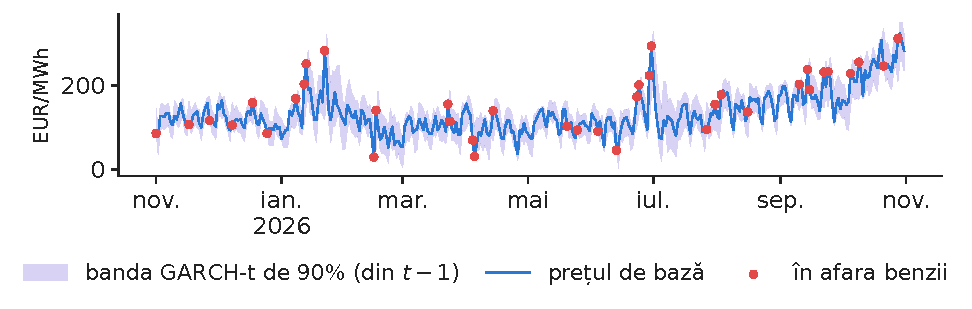
\includegraphics[width=\textwidth,height=0.416\textheight,keepaspectratio]{charts/ro/case_band.pdf}\end{center}\vspace{-3mm}
\chartsource{Sursa: energy-charts.info (OPCOM, prin ENTSO-E); estimări proprii. Date: anul de test 2025-11-01 - 2026-10-31.}
\vspace{0.5mm}
\begin{itemize}\setlength{\itemsep}{0pt}
  \item Banda = prețul prognozat $\pm$ cuantila Student $\times\hat\sigma_t$, stabilită în ziua $t-1$
    \begin{itemize}\setlength{\itemsep}{0pt}
      \item 38 din 365 de zile în afara benzii (10{,}4\%, față de 10\% așteptat): 9{,}4\% între noiembrie și aprilie, 11{,}4\% între mai și octombrie
      \item Semilățimea medie: 33 EUR/MWh în prima jumătate, 36 în septembrie--octombrie
    \end{itemize}
\end{itemize}
\par\vfill\manager{un furnizor își poate fixa limita zilnică de achiziție pe baza acestei benzi
    \begin{itemize}\setlength{\itemsep}{0pt}
      \item Testele formale ale acestor benzi se studiază în cursul 4.
    \end{itemize}}\par\vspace{0.5mm}
\par\vfill\noindent{\scriptsize\color{FooterGray}(estimare proprie)}\hfill\qlink{EMQA\_L3\_case\_band}{Quantlets/L3/EMQA_L3_case_band}\par\vspace{0.5mm}
\end{frame}

\begin{frame}{Studiu de caz: limitele pentru noiembrie 2026 și șocul din aprilie}
\small
\begin{center}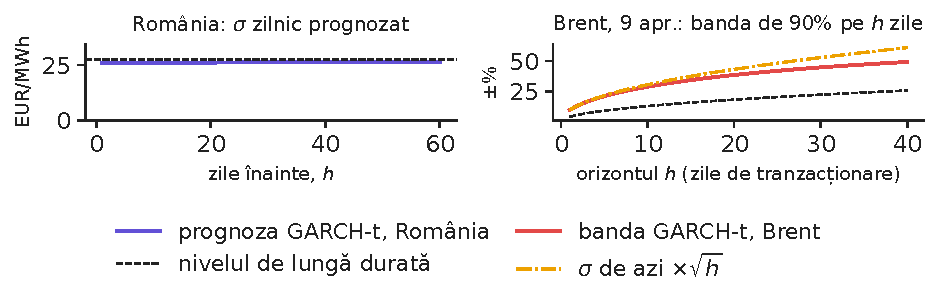
\includegraphics[width=\textwidth,height=0.471\textheight,keepaspectratio]{charts/ro/term_structure.pdf}\end{center}\vspace{-3mm}
\chartsource{Sursa: energy-charts.info (OPCOM, prin ENTSO-E); Yahoo Finance (Brent BZ=F, titlul SparkChange EUA ETC); EODHD (acțiuni BVB). Date: prognoze GARCH(1,1)-t făcute cu datele pînă la 2026-10-31.}
\vspace{0.5mm}
\begin{itemize}\setlength{\itemsep}{0pt}
  \item România, 31 octombrie 2026: $\hat\sigma$ = 26{,}0 EUR/MWh, aproape de nivelul de lungă durată, 27{,}6
    \begin{itemize}\setlength{\itemsep}{0pt}
      \item Limita de 90\% pentru o zi: circa $\pm$43 EUR/MWh în fiecare zi din noiembrie; Brent: banda crește mai lent decît $\sigma\sqrt{h}$
    \end{itemize}
\end{itemize}
\par\vfill\manager{stabiliți limitele după structura la termen a prognozei, nu după volatilitatea de azi.}\par\vspace{0.5mm}
\par\vfill\noindent{\scriptsize\color{FooterGray}(estimare proprie)}\hfill\qlink{EMQA\_L3\_term\_structure}{Quantlets/L3/EMQA_L3_term_structure}\par\vspace{0.5mm}
\end{frame}

\begin{frame}{Studiul de caz C3: acțiunile energetice, slab corelate cu petrolul}
\footnotesize
\begin{itemize}\setlength{\itemsep}{1pt}
  \item \textbf{Ce a făcut lucrarea} (Grecu, Cramer, Pele \& Lessmann, 2025)
    \begin{itemize}\setlength{\itemsep}{0pt}
      \item Date: indicii bursieri ai celor 27 de state ale Uniunii Europene, contractele futures pe Brent și TTF, 2010--2023
      \item Metodă: volatilitatea fiecărei serii cu un model GARCH, apoi o corelație condiționată dinamică (DCC) pentru fiecare zi; un model Markov pentru regimurile acestei corelații
      \item Rezultat: corelația cu petrolul este în general între 0 și 0{,}4; Europa Centrală și de Est (ECE) este regiunea cel mai slab corelată; regimurile persistă cu probabilitate de peste 98\%
    \end{itemize}
  \item \textbf{Replicarea noastră} (OMV Petrom, Romgaz (SNG), Nuclearelectrica (SNN) față de Brent, 2\,860 de zile)
    \begin{itemize}\setlength{\itemsep}{0pt}
      \item Parametrii DCC: $a$ = 0{,}021, $b$ = 0{,}950; corelația reacționează lent și este foarte persistentă
      \item Corelația medie: 0{,}13; maximum 0{,}54 în 2020, minimum \ensuremath{-}0{,}32 în 2022, aceeași cronologie ca în lucrare
      \item Acoperirea riscului coșului cu Brent, în afara eșantionului: variația varianței \ensuremath{-}1{,}7\% (dinamic), \ensuremath{-}6{,}9\% (static); valoare negativă = risc mai mare
    \end{itemize}
\end{itemize}
\par\vspace{0.5mm}{\scriptsize \begin{itemize}\setlength{\itemsep}{0pt}
  \item Cifrele C3 sînt calculate cu notebook-ul Jupyter al studiului de caz C3, pe datele noastre; rezultatele lucrării sînt prezentate în fișa studiului de caz.
\end{itemize}}
\par\vfill\manager{riscul acțiunilor energetice românești ține de reglementare și de piața locală
    \begin{itemize}\setlength{\itemsep}{0pt}
      \item Acoperirea cu Brent nu îl reduce.
    \end{itemize}}\par\vspace{0.5mm}
\par\vfill\noindent{\scriptsize\color{FooterGray}(Grecu, Cramer, Pele \& Lessmann, 2025, NAJEF; studiul de caz C3)}\par\vspace{0.5mm}
\end{frame}

\section*{Recapitulare}

\begin{frame}{Test 1: timpul de înjumătățire al unui șoc petrolier}
\small
\begin{itemize}
  \item Pentru Brent, GARCH(1,1)-t dă $\hat\alpha+\hat\beta$ = 0{,}973
    \begin{itemize}\setlength{\itemsep}{0pt}
      \item După un șoc, în cît timp dispare jumătate din varianța suplimentară?
    \end{itemize}
\end{itemize}
\vspace{2mm}
\begin{exampleblock}{R\u{a}spuns}
\begin{itemize}
  \item $h_{1/2}=\ln 0{,}5/\ln$ 0{,}973 = 25{,}6 zile lucrătoare, circa 5 săptămîni: limitele rămîn mai largi săptămîni întregi, nu cîteva zile.
\end{itemize}
\end{exampleblock}
\end{frame}

\begin{frame}{Test 2: procente sau euro}
\small
\begin{itemize}
  \item În 2022, volatilitatea procentuală a prețului din România a fost aceeași ca în 2019
    \begin{itemize}\setlength{\itemsep}{0pt}
      \item S-a schimbat riscul unei poziții deschise de 10 MW a unui furnizor?
    \end{itemize}
\end{itemize}
\vspace{2mm}
\begin{exampleblock}{R\u{a}spuns}
\begin{itemize}
  \item Da: poziția cîștigă sau pierde în euro, iar volatilitatea șocurilor în EUR/MWh a crescut de 4{,}1 ori, odată cu nivelul prețului.
\end{itemize}
\end{exampleblock}
\end{frame}

\begin{frame}{Test 3: creșterea de luni}
\small
\begin{itemize}
  \item Prețul PZU crește cu 35\% de duminică pînă luni
    \begin{itemize}\setlength{\itemsep}{0pt}
      \item Trebuie departamentul de risc să lărgească limitele?
    \end{itemize}
\end{itemize}
\vspace{2mm}
\begin{exampleblock}{R\u{a}spuns}
\begin{itemize}
  \item Nu: în medie, prețul de luni este cu 38\% mai mare decît cel de duminică
    \begin{itemize}\setlength{\itemsep}{0pt}
      \item Calendarul este inclus în ecuația mediei, iar în modelul GARCH intră doar șocul $\varepsilon_t$, aici aproape zero.
    \end{itemize}
\end{itemize}
\end{exampleblock}
\end{frame}

\begin{frame}{Test 4: alegerea modelului de volatilitate}
\small
\begin{itemize}
  \item Modelul de volatilitate al unui furnizor are cea mai mică eroare pătratică medie în anul de test, datorită a trei zile extreme
    \begin{itemize}\setlength{\itemsep}{0pt}
      \item Ce îi cereți?
    \end{itemize}
\end{itemize}
\vspace{2mm}
\begin{exampleblock}{R\u{a}spuns}
\begin{itemize}
  \item Valoarea QLIKE pe aceleași zile și un test DM față de GARCH-t și de varianța istorică pe 30 de zile
    \begin{itemize}\setlength{\itemsep}{0pt}
      \item În anul nostru de test, cel mai bun QLIKE în EUR/MWh îl are EGARCH-t, fără a fi semnificativ mai bun decît GARCH-t.
    \end{itemize}
\end{itemize}
\end{exampleblock}
\end{frame}

\begin{frame}{Test 5: după o creștere sau după o scădere}
\small
\begin{itemize}
  \item Ieri prețul s-a modificat cu 61 EUR/MWh
    \begin{itemize}\setlength{\itemsep}{0pt}
      \item Pentru un cumpărător, ziua de mîine este mai riscantă după o creștere sau după o scădere?
    \end{itemize}
\end{itemize}
\vspace{2mm}
\begin{exampleblock}{R\u{a}spuns}
\begin{itemize}
  \item După o creștere: modelul GJR în EUR/MWh dă $\sigma$ = 37{,}6 după o creștere și 30{,}6 după o scădere (efectul de levier invers).
\end{itemize}
\end{exampleblock}
\end{frame}

\begin{frame}{Recapitulare}
\small
\vspace{-2mm}\begin{multicols}{2}\scriptsize\tableofcontents[hideallsubsections]\end{multicols}
\begin{itemize}\setlength{\itemsep}{1pt}
  \item \textbf{Măsurare}
    \begin{itemize}\setlength{\itemsep}{0pt}
      \item Mai întîi se elimină calendarul săptămînal; în procente criza nu a fost mai volatilă, în EUR/MWh volatilitatea a fost de 4{,}1 ori mai mare
    \end{itemize}
  \item \textbf{Modelare și prognoză}
    \begin{itemize}\setlength{\itemsep}{0pt}
      \item GARCH-t este modelul implicit; șocurile petrolului se înjumătățesc în circa 5 săptămîni; cursul următor: măsurarea riscului în companiile energetice (cursul 4)
    \end{itemize}
\end{itemize}
\end{frame}

\begin{frame}{Cercetările grupului nostru despre volatilitate și risc}
\footnotesize
\begin{itemize}\setlength{\itemsep}{1pt}
  \item \textbf{Prețurile energiei și bursele din UE} (Grecu, Cramer, Pele \& Lessmann, 2025, NAJEF)
    \begin{itemize}\setlength{\itemsep}{0pt}
      \item Ce a făcut lucrarea: volatilitate GARCH, corelații DCC zilnice și regimuri Markov pentru 27 de indici naționali, față de petrol și gaze, 2010--2023
      \item Rezultat: piețele europene urmează mai mult petrolul decît gazele, cu regimuri persistente (studiul de caz C3)
    \end{itemize}
  \item \textbf{Entropia și riscul de piață} (Pele, Lazar \& Dufour, 2017, Entropy)
    \begin{itemize}\setlength{\itemsep}{0pt}
      \item Ce a făcut lucrarea: a măsurat entropia randamentelor intrazilnice euro--yen și a legat-o de valoarea expusă la risc (VaR) și de pierderea medie în coada distribuției (ES)
      \item Rezultat: o relație negativă între entropie și VaR, respectiv ES intrazilnic; entropia intrazilnică servește apoi la prognoza VaR zilnic
    \end{itemize}
  \item \textbf{Entropia datelor de înaltă frecvență și riscul zilnic} (Pele \& Mazurencu-Marinescu-Pele, 2019, Entropy)
    \begin{itemize}\setlength{\itemsep}{0pt}
      \item Ce a făcut lucrarea: a folosit entropia randamentelor intrazilnice ale Bitcoin pentru prognoza VaR zilnic, comparativ cu modelele GARCH clasice
      \item Rezultat: prognoza VaR bazată pe entropie dă cele mai bune rezultate la testare; datele intrazilnice conțin informație despre riscul zilnic
    \end{itemize}
  \item \textbf{Energy Financial Risk Meter} (Toma, Dima, Grecu, Pele \& Lessmann, 2026, SSRN)
    \begin{itemize}\setlength{\itemsep}{0pt}
      \item Ce a făcut lucrarea: un indicator al riscului sistemic pentru sectorul energetic din UE; tema cursului 4
    \end{itemize}
\end{itemize}
\par\vspace{0.5mm}{\scriptsize \begin{itemize}\setlength{\itemsep}{0pt}
  \item Rezultatele de pe acest diapozitiv sînt cele raportate în lucrări; celelalte cifre din curs provin din calculele noastre.
\end{itemize}}
\par\vfill\noindent{\scriptsize\color{FooterGray}(Academia de Studii Economice din București; Academia Română, Institutul de Prognoză Economică)}\par\vspace{0.5mm}
\end{frame}

\begin{frame}{AIDA 2026: crizele geopolitice fac negativă legătura burselor din UE cu energia}
\footnotesize
\begin{itemize}\setlength{\itemsep}{1pt}
  \item \textbf{Ce a făcut lucrarea} (A.-A.\ Cramer, conferința AIDA (AI and Digital Assets in Energy and Finance), 3 iunie 2026)
    \begin{itemize}\setlength{\itemsep}{0pt}
      \item Date: indicii bursieri ai țărilor din UE, pe regiuni și după industrializare; futures pe Brent și TTF, 2010--2026
      \item Modele: GARCH, apoi corelația DCC zilnică (ca în studiul de caz C3); regimuri Markov; răspunsul la șocuri
    \end{itemize}
  \item \textbf{Ce a găsit}
    \begin{itemize}\setlength{\itemsep}{0pt}
      \item Corelația cu petrolul: în general pozitivă, de cele mai multe ori între 0 și 0{,}4; cu gazele, mai mică
      \item Petrolul contează mai ales în sudul și vestul Europei, gazele în nord și vest; țările industrializate urmează mai mult petrolul
      \item Crizele fac corelația negativă: Crimeea, 2014 (gaze), Ucraina, 2022 (gaze: cel mai puternic în ECE), Orientul Mijlociu, 2026
      \item După un șoc, bursele țărilor celor mai industrializate sînt mai afectate în primele luni, apoi efectul se estompează
    \end{itemize}
\end{itemize}
\par\vspace{0.5mm}{\scriptsize \begin{itemize}\setlength{\itemsep}{0pt}
  \item Rezultatele sînt cele raportate de autori. Prezentarea: \href{https://github.com/danpele/EMQA/blob/main/resources/aida2026/cramer_energy_stock_markets.pdf}{diapozitive}; articolul: \href{https://doi.org/10.1016/j.najef.2025.102420}{doi:10.1016/j.najef.2025.102420}.
\end{itemize}}
\par\vfill\manager{cine acoperă acțiuni din UE cu futures pe petrol sau gaze trebuie să se aștepte ca, în criză, corelația să își schimbe semnul.}\par\vspace{0.5mm}
\par\vfill\noindent{\scriptsize\color{FooterGray}(Cramer, conferința AIDA, București, 3 iunie 2026; Grecu, Cramer, Pele \& Lessmann, 2025, NAJEF)}\par\vspace{0.5mm}
\end{frame}

\begin{frame}{AIDA 2026: șocurile tokenurilor energetice se transmit mai ales pe termen scurt}
\footnotesize
\begin{itemize}\setlength{\itemsep}{1pt}
  \item \textbf{Ce a făcut lucrarea} (S.\ Ben Amor și M.\ Horváth, conferința AIDA, 4 iunie 2026)
    \begin{itemize}\setlength{\itemsep}{0pt}
      \item Date: tokenuri energetice (Power Ledger, SunContract, Energy Web), criptomonede, acțiuni de energie curată, petrol, gaze, certificate de emisii, obligațiuni verzi; dec.\ 2020 -- ian.\ 2026
      \item Metodă: model vectorial autoregresiv cu parametri variabili în timp; transmiterea șocurilor, separată pe termen scurt (tranzitorie) și lung (persistentă)
    \end{itemize}
  \item \textbf{Ce a găsit}
    \begin{itemize}\setlength{\itemsep}{0pt}
      \item Interconectarea: circa 60\% din total pe termen scurt, circa 5\% pe termen lung
      \item Crizele (criptomonede, 2021; energie, 2022) amplifică șocurile pe termen scurt; pe termen lung, structura rămîne stabilă
      \item Power Ledger și SunContract transmit cel mai mult pe termen scurt; Energy Web contează mai ales în crize
      \item Diversificarea depinde de token: portofoliul de varianță minimă, raport Sharpe 0{,}127 fără tokenuri, 0{,}143 cu SunContract
    \end{itemize}
\end{itemize}
\par\vspace{0.5mm}{\scriptsize \begin{itemize}\setlength{\itemsep}{0pt}
  \item Rezultatele sînt cele raportate de autori. Prezentarea: \href{https://github.com/danpele/EMQA/blob/main/resources/aida2026/benamor_energy_tokens_spillovers.pdf}{diapozitive}.
\end{itemize}}
\par\vfill\manager{șocurile se transmit în cîteva zile
    \begin{itemize}\setlength{\itemsep}{0pt}
      \item Valoarea pentru diversificare se judecă pentru fiecare token în parte.
    \end{itemize}}\par\vspace{0.5mm}
\par\vfill\noindent{\scriptsize\color{FooterGray}(Ben Amor și Horváth, conferința AIDA, București, 4 iunie 2026)}\par\vspace{0.5mm}
\end{frame}

\begin{frame}{Lecturi și resurse suplimentare}
\small
\begin{columns}[T,onlytextwidth]
\begin{column}{0.52\textwidth}
\begin{itemize}\setlength{\itemsep}{1pt}
  \item \textbf{R.\,F.\ Engle, GARCH 101} (2001): cea mai clară introducere scurtă, scrisă de laureatul Nobel care a propus modelul ARCH --- \href{https://doi.org/10.1257/jep.15.4.157}{doi:10.1257/jep.15.4.157}.
  \item \textbf{R.\ Weron, Modeling and Forecasting Electricity Loads and Prices} (Wiley, 2006): faptele stilizate și volatilitatea prețurilor energiei electrice --- \href{https://doi.org/10.1002/9781118673362}{doi:10.1002/9781118673362}.
  \item \textbf{Pachetul Python \texttt{arch}} (K.\ Sheppard), folosit pentru toate modelele din acest curs: \href{https://arch.readthedocs.io}{arch.readthedocs.io}.
\end{itemize}
\end{column}
\begin{column}{0.45\textwidth}
\begin{itemize}\setlength{\itemsep}{1pt}
  \item \textbf{Acest curs}: cod, date, notebook-uri Jupyter --- \href{https://github.com/danpele/EMQA}{github.com/danpele/EMQA}.
  \item \textbf{Studiul de caz C3}: modelul DCC și acoperirea cu Brent pentru acțiunile energetice românești, pas cu pas.
  \item \textbf{Exercițiu practic}: notebook-ul Jupyter reproduce toate graficele și cifrele din acest curs --- \href{\emqarepo/\emqanb}{notebooks/}.
\end{itemize}
\end{column}
\end{columns}
\end{frame}

\begin{frame}{Bibliografie (1/3)}
\scriptsize
\begin{itemize}\setlength{\itemsep}{1pt}\scriptsize
\item Andersen, T.\,G.\ \& Bollerslev, T.\ (1998). Answering the skeptics: Yes, standard volatility models do provide accurate forecasts. \textit{International Economic Review}, 39(4), 885--905. \href{https://doi.org/10.2307/2527343}{doi:10.2307/2527343}
\item Ben Amor, S.\ \& Horváth, M.\ (2026). Transitory and persistent cross-market spillovers of energy tokens. AIDA Conference, Bucharest University of Economic Studies, 4 June 2026. \href{https://github.com/danpele/EMQA/blob/main/resources/aida2026/benamor_energy_tokens_spillovers.pdf}{github.com/danpele/EMQA/resources/aida2026}
\item Bollerslev, T.\ (1986). Generalized autoregressive conditional heteroskedasticity. \textit{Journal of Econometrics}, 31(3), 307--327. \href{https://doi.org/10.1016/0304-4076(86)90063-1}{doi:10.1016/0304-4076(86)90063-1}
\item Bollerslev, T.\ (1987). A conditionally heteroskedastic time series model for speculative prices and rates of return. \textit{Review of Economics and Statistics}, 69(3), 542--547. \href{https://doi.org/10.2307/1925546}{doi:10.2307/1925546}
\item Corsi, F.\ (2009). A simple approximate long-memory model of realized volatility. \textit{Journal of Financial Econometrics}, 7(2), 174--196. \href{https://doi.org/10.1093/jjfinec/nbp001}{doi:10.1093/jjfinec/nbp001}
\item Cramer, A.-A.\ (2026). The link between energy prices and stock markets in European Union countries (with R.-A.\ Grecu, D.\,T.\ Pele and S.\ Lessmann). AIDA Conference, Bucharest University of Economic Studies, 3 June 2026. \href{https://github.com/danpele/EMQA/blob/main/resources/aida2026/cramer_energy_stock_markets.pdf}{github.com/danpele/EMQA/resources/aida2026}
\item Diebold, F.\,X.\ \& Mariano, R.\,S.\ (1995). Comparing predictive accuracy. \textit{Journal of Business \& Economic Statistics}, 13(3), 253--263. \href{https://doi.org/10.1080/07350015.1995.10524599}{doi:10.1080/07350015.1995.10524599}
\item Engle, R.\,F.\ (1982). Autoregressive conditional heteroscedasticity with estimates of the variance of United Kingdom inflation. \textit{Econometrica}, 50(4), 987--1007. \href{https://doi.org/10.2307/1912773}{doi:10.2307/1912773}
\end{itemize}
\end{frame}

\begin{frame}{Bibliografie (2/3)}
\scriptsize
\begin{itemize}\setlength{\itemsep}{1pt}\scriptsize
\item Engle, R.\,F.\ (2001). GARCH 101: The use of ARCH/GARCH models in applied econometrics. \textit{Journal of Economic Perspectives}, 15(4), 157--168. \href{https://doi.org/10.1257/jep.15.4.157}{doi:10.1257/jep.15.4.157}
\item Engle, R.\,F.\ \& Ng, V.\,K.\ (1993). Measuring and testing the impact of news on volatility. \textit{Journal of Finance}, 48(5), 1749--1778. \href{https://doi.org/10.1111/j.1540-6261.1993.tb05127.x}{doi:10.1111/j.1540-6261.1993.tb05127.x}
\item Glosten, L.\,R., Jagannathan, R.\ \& Runkle, D.\,E.\ (1993). On the relation between the expected value and the volatility of the nominal excess return on stocks. \textit{Journal of Finance}, 48(5), 1779--1801. \href{https://doi.org/10.1111/j.1540-6261.1993.tb05128.x}{doi:10.1111/j.1540-6261.1993.tb05128.x}
\item Grecu, R.\,A., Cramer, A.\,A., Pele, D.\,T.\ \& Lessmann, S.\ (2025). The link between energy prices and stock markets in European Union countries. \textit{North American Journal of Economics and Finance}, 78, 102420. \href{https://doi.org/10.1016/j.najef.2025.102420}{doi:10.1016/j.najef.2025.102420}
\item Hamilton, J.\,D.\ (1989). A new approach to the economic analysis of nonstationary time series and the business cycle. \textit{Econometrica}, 57(2), 357--384. \href{https://doi.org/10.2307/1912559}{doi:10.2307/1912559}
\item Hansen, P.\,R.\ \& Lunde, A.\ (2005). A forecast comparison of volatility models: Does anything beat a GARCH(1,1)? \textit{Journal of Applied Econometrics}, 20(7), 873--889. \href{https://doi.org/10.1002/jae.800}{doi:10.1002/jae.800}
\item Knittel, C.\,R.\ \& Roberts, M.\,R.\ (2005). An empirical examination of restructured electricity prices. \textit{Energy Economics}, 27(5), 791--817. \href{https://doi.org/10.1016/j.eneco.2004.11.005}{doi:10.1016/j.eneco.2004.11.005}
\item Lamoureux, C.\,G.\ \& Lastrapes, W.\,D.\ (1990). Persistence in variance, structural change, and the GARCH model. \textit{Journal of Business \& Economic Statistics}, 8(2), 225--234. \href{https://doi.org/10.1080/07350015.1990.10509794}{doi:10.1080/07350015.1990.10509794}
\end{itemize}
\end{frame}

\begin{frame}{Bibliografie (3/3)}
\scriptsize
\begin{itemize}\setlength{\itemsep}{1pt}\scriptsize
\item Ljung, G.\,M.\ \& Box, G.\,E.\,P.\ (1978). On a measure of lack of fit in time series models. \textit{Biometrika}, 65(2), 297--303. \href{https://doi.org/10.1093/biomet/65.2.297}{doi:10.1093/biomet/65.2.297}
\item Nelson, D.\,B.\ (1991). Conditional heteroskedasticity in asset returns: A new approach. \textit{Econometrica}, 59(2), 347--370. \href{https://doi.org/10.2307/2938260}{doi:10.2307/2938260}
\item Patton, A.\,J.\ (2011). Volatility forecast comparison using imperfect volatility proxies. \textit{Journal of Econometrics}, 160(1), 246--256. \href{https://doi.org/10.1016/j.jeconom.2010.03.034}{doi:10.1016/j.jeconom.2010.03.034}
\item Pele, D.\,T., Lazar, E.\ \& Dufour, A.\ (2017). Information entropy and measures of market risk. \textit{Entropy}, 19(5), 226. \href{https://doi.org/10.3390/e19050226}{doi:10.3390/e19050226}
\item Pele, D.\,T.\ \& Mazurencu-Marinescu-Pele, M.\ (2019). Using high-frequency entropy to forecast Bitcoin's daily value at risk. \textit{Entropy}, 21(2), 102. \href{https://doi.org/10.3390/e21020102}{doi:10.3390/e21020102}
\item RiskMetrics (1996). \textit{RiskMetrics --- Technical Document}, 4th ed. J.\,P.\ Morgan / Reuters, New York. \href{https://www.msci.com/documents/10199/5915b101-4206-4ba0-aee2-3449d5c7e95a}{msci.com}
\item Toma, F.-M., Dima, D.-M., Grecu, R., Pele, D.\,T.\ \& Lessmann, S.\ (2026). Energy Financial Risk Meter: Systemic risk in the EU energy sector. SSRN Working Paper 6985301. \href{https://doi.org/10.2139/ssrn.6985301}{doi:10.2139/ssrn.6985301}
\item Uniejewski, B., Weron, R.\ \& Ziel, F.\ (2018). Variance stabilizing transformations for electricity spot price forecasting. \textit{IEEE Transactions on Power Systems}, 33(2), 2219--2229. \href{https://doi.org/10.1109/TPWRS.2017.2734563}{doi:10.1109/TPWRS.2017.2734563}
\item Weron, R.\ (2006). \textit{Modeling and Forecasting Electricity Loads and Prices: A Statistical Approach}. Wiley, Chichester. \href{https://doi.org/10.1002/9781118673362}{doi:10.1002/9781118673362}
\item Weron, R.\ (2014). Electricity price forecasting: A review of the state-of-the-art with a look into the future. \textit{International Journal of Forecasting}, 30(4), 1030--1081. \href{https://doi.org/10.1016/j.ijforecast.2014.08.008}{doi:10.1016/j.ijforecast.2014.08.008}
\end{itemize}
\end{frame}

\appendix

\section*{Anexă}

\begin{frame}{Anexa A: funcția de verosimilitate Student a modelului GARCH}
\footnotesize
\begin{columns}[T,onlytextwidth]
\begin{column}{0.56\textwidth}
\[ \begin{aligned}\ell(\theta)=\sum_{t=1}^{T}\Bigl[&\ln\Gamma\bigl(\tfrac{\nu+1}{2}\bigr)-\ln\Gamma\bigl(\tfrac{\nu}{2}\bigr)-\tfrac12\ln\bigl(\pi(\nu-2)\bigr)\\ &-\tfrac12\ln\sigma_t^2-\tfrac{\nu+1}{2}\ln\Bigl(1+\frac{\varepsilon_t^2}{(\nu-2)\sigma_t^2}\Bigr)\Bigr]\end{aligned} \]\begin{itemize}\setlength{\itemsep}{1pt}
  \item $\theta=(\omega,\alpha,\beta,\nu)$
    \begin{itemize}\setlength{\itemsep}{0pt}
      \item $\Gamma$ = funcția gamma
      \item Factorul $\nu-2$ dă variabilei Student varianța 1.
    \end{itemize}
  \item Maximizare numerică cu $\omega>0$, $\alpha,\beta\ge0$, $\alpha+\beta<1$, $\nu>2$
    \begin{itemize}\setlength{\itemsep}{0pt}
      \item Erori standard robuste
      \item Pachetul \texttt{arch}.
    \end{itemize}
  \item Cazul normal: $\ell=-\tfrac12\sum_t\bigl[\ln(2\pi)+\ln\sigma_t^2+\varepsilon_t^2/\sigma_t^2\bigr]$, limita pentru $\nu\to\infty$.
\end{itemize}
\end{column}
\begin{column}{0.41\textwidth}
{\scriptsize\renewcommand{\arraystretch}{1.2}\setlength{\tabcolsep}{4pt}
\begin{tabular}{@{}lrr@{}}\toprule
GARCH(1,1)-t & \% & EUR/MWh \\ \midrule
$\omega$ & 105{,}677 (35{,}482) & 4{,}635 (1{,}773) \\
$\alpha$ & 0{,}308 (0{,}081) & 0{,}102 (0{,}020) \\
$\beta$ & 0{,}438 (0{,}150) & 0{,}892 (0{,}021) \\
$\nu$ & 4{,}266 (0{,}370) & 6{,}149 (0{,}655) \\
\bottomrule\end{tabular}}
\par\vspace{0.5mm}{\scriptsize \begin{itemize}\setlength{\itemsep}{0pt}
  \item Estimația (eroarea standard).
\end{itemize}}
\end{column}
\end{columns}
\par\vfill\noindent{\scriptsize\color{FooterGray}(Bollerslev, 1987, RESTAT)}\par\vspace{0.5mm}
\end{frame}

\begin{frame}{Anexa B: prognoza pe mai mulți pași și timpul de înjumătățire}
\small
\begin{itemize}\setlength{\itemsep}{1pt}
  \item \textbf{Pasul 1}
    \begin{itemize}\setlength{\itemsep}{0pt}
      \item Scriem $\varepsilon_{t}^2=\sigma_{t}^2+v_t$, cu $\E_{t-1}[v_t]=0$; atunci $\sigma^2_{t+1}=\omega+(\alpha+\beta)\sigma_t^2+\alpha v_t$
    \end{itemize}
  \item \textbf{Pasul 2}
    \begin{itemize}\setlength{\itemsep}{0pt}
      \item Aplicăm media condiționată în $T$: $\E_T[\sigma^2_{T+h}]=\omega+(\alpha+\beta)\E_T[\sigma^2_{T+h-1}]$, pentru $h\ge2$
      \item Scădem $\bar\sigma^2=\omega+(\alpha+\beta)\bar\sigma^2$: abaterea față de $\bar\sigma^2$ se înmulțește în fiecare zi cu $\alpha+\beta$
    \end{itemize}
  \item \textbf{Pasul 3}
    \begin{itemize}\setlength{\itemsep}{0pt}
      \item Rezultă $\E_T[\sigma^2_{T+h}]-\bar\sigma^2=(\alpha+\beta)^{h-1}(\sigma^2_{T+1}-\bar\sigma^2)$
      \item Rămîne jumătate din abatere cînd $(\alpha+\beta)^{h}=1/2$, deci $h_{1/2}=\ln(1/2)/\ln(\alpha+\beta)$
    \end{itemize}
  \item \textbf{GJR și EGARCH}
    \begin{itemize}\setlength{\itemsep}{0pt}
      \item GJR cu $z_t$ simetric: persistența este $\alpha+\gamma/2+\beta$, deoarece $\Pr(\varepsilon<0)=1/2$
      \item EGARCH: $\ln\sigma_t^2$ urmează un proces autoregresiv cu coeficientul $\beta$; persistența este $\beta$
    \end{itemize}
\end{itemize}
\par\vfill\noindent{\scriptsize\color{FooterGray}(Engle, 2001, JEP; Bollerslev, 1986, JOE)}\par\vspace{0.5mm}
\end{frame}

\begin{frame}{Anexa C: cele șase modele, în ambele unități de măsură}
\small
\begin{center}{\footnotesize\renewcommand{\arraystretch}{1.15}\setlength{\tabcolsep}{4pt}
\begin{tabular}{@{}lrrrrrr@{}}\toprule
Modelul & log-L, \% & AIC, \% & BIC, \% & log-L, EUR & AIC, EUR & BIC, EUR \\ \midrule
GARCH, normal & \ensuremath{-}12\,360{,}3 & 24\,726{,}6 & 24\,744{,}5 & \ensuremath{-}12\,274{,}7 & 24\,555{,}4 & 24\,573{,}2 \\
GARCH, Student & \ensuremath{-}12\,094{,}5 & 24\,197{,}0 & 24\,220{,}8 & \ensuremath{-}12\,209{,}4 & 24\,426{,}8 & 24\,450{,}7 \\
GJR, normal & \ensuremath{-}12\,329{,}4 & 24\,666{,}8 & 24\,690{,}7 & \ensuremath{-}12\,246{,}6 & 24\,501{,}3 & 24\,525{,}1 \\
GJR, Student & \ensuremath{-}12\,087{,}2 & 24\,184{,}3 & 24\,214{,}1 & \ensuremath{-}12\,185{,}9 & 24\,381{,}9 & 24\,411{,}7 \\
EGARCH, normal & \ensuremath{-}12\,329{,}8 & 24\,667{,}6 & 24\,691{,}4 & \ensuremath{-}12\,243{,}1 & 24\,494{,}2 & 24\,518{,}0 \\
EGARCH, Student & \ensuremath{-}12\,089{,}7 & 24\,189{,}4 & 24\,219{,}2 & \ensuremath{-}12\,182{,}1 & 24\,374{,}1 & 24\,403{,}9 \\
\bottomrule\end{tabular}}\end{center}
\par\vspace{0.5mm}{\scriptsize \begin{itemize}\setlength{\itemsep}{0pt}
  \item log-L = log-verosimilitatea $\hat\ell$; AIC $=2k-2\hat\ell$, BIC $=k\ln T-2\hat\ell$, $k$ = numărul de parametri; 2\,853 de zile, 1 ianuarie 2019 -- 31 octombrie 2026.
  \item Asimetria $\hat\gamma$ și $\hat\nu$: GJR-t 0{,}225, 4{,}41 (\%); \ensuremath{-}0{,}127, 6{,}50 (EUR/MWh).
\end{itemize}}
\par\vfill\noindent{\scriptsize\color{FooterGray}(Glosten, Jagannathan \& Runkle, 1993; Nelson, 1991)}\par\vspace{0.5mm}
\end{frame}

\begin{frame}{Anexa D: filtrul Hamilton și robustețea funcției QLIKE}
\small
\begin{itemize}\setlength{\itemsep}{1pt}
  \item \textbf{Filtrul Hamilton} (modelul Markov)
    \begin{itemize}\setlength{\itemsep}{0pt}
      \item Predicția: $\Pr(s_t=j\mid\mathcal F_{t-1})=\sum_i p_{ij}\Pr(s_{t-1}=i\mid\mathcal F_{t-1})$
      \item Actualizarea: se înmulțește cu densitatea normală a lui $u_t$ în regimul $j$ și se normalizează; suma logaritmilor constantelor de normalizare este log-verosimilitatea
      \item Probabilitățile netezite (din grafic) folosesc toate datele, cele filtrate doar trecutul; o avertizare în timp real trebuie să folosească probabilitățile filtrate
    \end{itemize}
  \item \textbf{De ce QLIKE}
    \begin{itemize}\setlength{\itemsep}{0pt}
      \item Dacă $\E_{t-1}[\varepsilon_t^2]=\sigma_t^2$, valoarea așteptată a QLIKE este minimă numai pentru $\hat\sigma_t^2=\sigma_t^2$, oricît de zgomotos ar fi $\varepsilon_t^2$
      \item Același lucru este valabil pentru MSE; alte funcții, ca $|\varepsilon_t|-\hat\sigma_t$ sau erorile logaritmice, pot ordona greșit modelele (Patton, 2011)
      \item Statistica DM: media diferențelor zilnice de pierdere împărțită la eroarea ei standard Newey--West (7 decalaje); asimptotic normală
    \end{itemize}
\end{itemize}
\par\vfill\noindent{\scriptsize\color{FooterGray}(Hamilton, 1989; Patton, 2011, JOE; Diebold \& Mariano, 1995)}\par\vspace{0.5mm}
\end{frame}

\end{document}
